% TFG - José Ángel Martín Baos. Escuela Superior de Informática. 2017
\documentclass[twoside]{esi-tfg}
\usepackage{custom}
% TFG - José Ángel Martín Baos. Escuela Superior de Informática. 2017
%% -- Información general --
\title{Nombre del TFG} % TODO
\author{José Ángel Martín Baos}{}


%% -- Variables de la clase esi-tfg --

%- datos del autor

%\address{}
%\city{Ciudad Real}
%\country{Spain}
\email{JoseAngel.Martin3@alu.uclm.es}
\phone{696 836 882}
% \homepage{http://esi.uclm.es/~juan.nadie}


%- datos del documento

%\logo{informatica.pdf}
\advisorFirst{Dr. Luis Rodríguez Benítez}
\advisorDepartment{Tecnologías y Sistemas de Información}
\advisorSecond{Dr. Ricardo García Ródenas}
\docdate{2017}{Junio} % TODO
\intensification{Ingeniería de Computadores}
%\license{Texto de licencia al gusto de cada uno.}




\begin{document}
	% TODO: Memoria en ingles
	% Español: Resumen, Indroducción y conclusiones

  % Notas al pie de pagina con: \footnote{Sí, los agradecimientos se firman} 

\cover
\bastardtitle
\frontpage

\frontmatter
\copyrightpage
\jury

% TFG - José Ángel Martín Baos. Escuela Superior de Informática. 2018
% !TeX spellcheck = es_ES

\chapter{Abstract}

Road transport is the recognized major source of air pollution in urban areas, with detrimental effects on the local air quality, ecology, and even on human health. For this reason there is an increasing need to estimate precisely its contribution to air pollution on the cities. Dynamic Traffic Management (DTM) systems are used to reduce the negative externalities of the traffic congestion. Nonetheless, the use of these systems require reliable mathematical emissions models and traffic and environmental monitoring infrastructures. Moreover, cities are distributed environments where events occur in real time and on a massive scale. Hence, intelligent systems capable of monitoring environmental and traffic parameters using distributed sensors to predict the pollution levels and recommend several palliative actions are needed.

This Bachelor of Science thesis aims to design and build a prototype of a low-cost distributed Internet of Things (IoT) system for monitoring the traffic flow and different environmental parameters such as temperature, pressure, humidity and several pollutant gases. This information is uploaded to a cloud service where it is processed. In addition, a web page is developed where the data collected by the different sensors can be monitored in real-time. Moreover, the web page also contains an alert system to inform the transport authority if a concrete parameter get over a pre-defined threshold and a historical section where the data collected in a certain time interval is shown.


\chapter{Resumen}

El transporte por carretera es la principal fuente de contaminación atmosférica en las zonas urbanas, con efectos perjudiciales sobre la calidad del aire, la ecología e incluso sobre la salud humana. Por esta razón, hay una creciente necesidad de estimar con precisión su contribución a la contaminación del aire en las ciudades. Los sistemas de Gestión Dinámica del Tráfico (DTM por sus siglas en inglés) se utilizan para la gestión y control del tráfico, y así poder reducir las externalidades negativas de la congestión. No obstante, el uso de estos sistemas requiere de modelos matemáticos confiables de emisiones y de infraestructuras de control de tráfico y de medio ambiente. Además, las ciudades son entornos distribuidos donde los eventos ocurren en tiempo real y de manera masiva. Por ello, se necesitan sistemas inteligentes capaces de monitorizar los parámetros ambientales y de tráfico utilizando sensores distribuidos para predecir los niveles de contaminación y recomendar diferentes acciones paliativas.

Este Trabajo Fin de Grado (TFG) tiene como objetivo el diseño y construcción de un prototipo de sistema distribuido del Internet de las Cosas (IoT por sus siglas en inglés) de bajo coste que permita monitorizar el flujo de tráfico y diferentes parámetros ambientales tales como la temperatura, presión, humedad y varios gases contaminantes. Esta información se envía a un servicio en la nube donde será procesada. Además, se ha desarrollado una página web donde se muestran en tiempo real los datos recopilados por los diferentes sensores. Esta página web también contiene un sistema de alerta para informar a la autoridad de transporte si un parámetro concreto supera un umbral predefinido, así como una sección donde los datos recopilados en un intervalo de tiempo son mostrados de forma gráfica.





% TFG - José Ángel Martín Baos. Escuela Superior de Informática. 2017
\chapter{Agradecimientos} % TODO

Agradecimientos ...

\quoteauthor{José Ángel}



\chapter{Acknowledgements} % TODO

Agradecimientos ...

\quoteauthor{José Ángel}

\dedication{Cita ...} % TODO

\tableofcontents
\listoftables
\listoffigures
\lstlistoflistings
% TFG - José Ángel Martín Baos. Escuela Superior de Informática. 2018
\chapter{List of Acronyms}

{\small
\begin{acronym}[XXXXXXXX]
	\acro{AES}		{Advanced Encryption Standard}
	\acro{ADC}		{Analogue to Digital Converter}
	\acro{BSc.}		{Bachelor of Science}
	\acro{CPU}		{Central Processing Unit}
	\acro{CITEAIR}	{Common Information to European Air}
	\acro{DSS}		{Decision Support System}
	\acro{DTM}		{Dynamic Traffic Management}
	\acro{EEA}		{European Environment Agency}
	\acro{ESA}		{European Space Agency}
	\acro{FPS}		{Frames Per Second}
	\Acro{GNU}     	{\acs{GNU} is Not Unix}
	\acro{GPU}		{Graphics Processing Unit}
	\acro{ITS}		{Intelligent Transportation Systems}
	\acro{IoT} 		{Internet of Things}
	\acro{OO}		{Object Oriented}
	\acro{OS}		{Operating System}
	\acro{PaaS}		{Platform as a Service}
	\acro{PWM}		{Pulse-Width Modulation}
	\acro{QoS}		{Quality of Service}
	\acro{SPI}		{Serial Peripheral Interface}
	\acro{SQL}		{Structured Query Language}
	\acro{SAD}		{Sum of Absolute Differences}
	\acro{TFG}		{Trabajo Fin de Grado}
	\acro{UUID}		{Universally Unique Identifier}
	\acro{UCLM}		{University of Castilla-La Mancha}
\end{acronym}
}


\mainmatter

% TFG - José Ángel Martín Baos. Escuela Superior de Informática. 2018
%%%% CHAPTER: Introducción %%%

%%% CHAPTER: Introduction %%%
\chapter{Introduction} % TODO: Revise
\drop{R}{oad} transportation is often the main source of air pollution in urban areas with detrimental effects on local air quality, ecology, and human health. Therefore, there is an increasing need to estimate precisely the contribution of road transport to air pollution in the cities, so that pollution-reduction measures can be designed and implemented appropriately \cite{SNB10}. These pollution-reduction measures are becoming increasingly relevant due to the continued growth in vehicle use and the deterioration in driving conditions (congestion). Many authorities find it difficult to meet their environmental targets (e.g. air quality standards or national emission ceilings) and, therefore, reliable emission models are needed, in order to predict accurately the impact of road transport on air pollution.

Therefore, intelligent cities are essential to prevent situations of high level contamination and take measures when these situations occur. These cities must predict the pollution peaks and take palliative measures, such as restricting the traffic to a number of vehicles, by the license plates, closing traffic in some streets, lowering the speed limits, etc. Moreover, traffic flows must be monitored as they affect the pollution levels in that city. For this reason, these cities must rely on an \ac{IoT} infrastructure connected to a cloud platform that supports those systems as well as sensor-based big data applications. \cite{Bib18}.

Typical pollution surveillance and control systems are composed of big and expensive devices that are only located in some points in a city, hence, they provide information for vast areas and sometimes those systems are not scalable. However, cities are distributed environments where the events occur in real time and on a massive scale. Therefore, an inexpensive distributed IoT architecture is needed to control pollution levels by zones or streets. These can be combined with a traffic surveillance infrastructure in order to have a complete system that could be used as a \ac{DSS} to help authorities to take decisions about environmental problems caused by pollution before they occur.

The objective in this \ac{BSc.} thesis is to design and build a prototype of an integrated low-cost road traffic and air pollution monitoring platform. It will only focus on the design and implementation of the software and hardware architecture that must allow the future implementation of an intelligent system for the prediction of the pollution levels, the recommendation of palliative actions and monitoring those actions. An inexpensive embedded system will be used for designing the architecture in order to obtain a scalable system not only in size but also in cost.


\begin{figure}[!h]
	\begin{center}
		\includegraphics[width=1\textwidth]{2-system_architecture.pdf}	
		\caption{System architecture}
		\label{fig:2-system_architecture}
	\end{center}
\end{figure}

%TODO: La introducción debe ser una presentación de los objetivos, en la cual se introduzcan todos los conceptos que aparezcan en la sección de objetivos.

% Contar que se va a usar el video en tiempo real para detectar los coches

% Hablar sobre el cloud

% Hablar sobre los terminos del O.4


\section{Document structure}

This section describes how the rest of the document is organized. To this end, each of the subsequent chapters is briefly presented.

\begin{definitionlist}
	\item[Chapter \ref{chap:objectives}: \nameref{chap:objectives}] In this chapter the different general and specific objectives that will be addressed in this work are defined.
	
	\item[Chapter \ref{chap:background}: \nameref{chap:background}] For the development of this \ac{BSc.} thesis a bibliographic research has been carried out. Firstly, an introduction about traffic flows and traffic emissions monitoring systems is discussed. In addition, some European projects which aims to measure and control de pollution generated are described. Then, an introduction is made about embedded systems and how they can be implemented in traffic and environmental surveillance. Raspberry Pi embedded systems are going to be used in this thesis, therefore their features and uses are described here. To finish with, it will go on to explain H.264/AVC video format, which is going to be used to measure the traffic flow using a camera.
	
	\item[Chapter \ref{chap:methodology}: \nameref{chap:methodology}] In this chapter the working methodology used to develop this \ac{BSc.} thesis is explained. To this effect, Scrum has been used as project management methodology and Kanban to control the progress of the project. In addition, the iterative and incremental software development methodology is used. To end with, the different physical and software resources required to perform this work are defined.
	
	\item[Chapter \ref{chap:results}: \nameref{chap:results}] In this chapter the work planning is presented. Subsequently, the different results and artefacts obtained from applying the methodology presented in the previous chapter, as well as the inconveniences produced during the project realization are described. 
	
	\item[Chapter \ref{chap:conclusions}: \nameref{chap:conclusions}] In this chapter the main milestones achieved during the execution of this project are described. In addition, a set of improvements and proposals for future work are commented. 
	%\REDNOTE{It will go on to make a brief reflection about the knowledge acquired during the realization of this work.}
	
	\item[Appendix \ref{chap:installation_guide}: \nameref{chap:installation_guide}] In this appendix the different steps needed to install and configure Raspberry Pi are described. This Appendix include the installation of the Raspbian Operating System in the Raspberry Pi, as well as the installation of the different sensors and libraries.
	
	\item[Appendix \ref{chap:config_file}: \nameref{chap:config_file}] In this appendix the configuration file used by the different Raspberry Pi devices is described.
\end{definitionlist}



\chapter{Introducción} % TODO
%%%%%
% \drop{I}{n}


\section{Estructura del documento}
En esta sección se describe como está organizado el resto del documento. Para ello se presenta brevemente cada uno de los capítulos posteriores.

\begin{definitionlist}
	\item[Capítulo \ref{chap:objectives}: \nameref{chap:objectives}] En este capítulo los diferentes objetivos generales y específicos que se pretenden abordar en este trabajo son definidos.
	
	\item[Capítulo \ref{chap:background}: \nameref{chap:background}] \REDNOTE{Explicar...}
	
	\item[Capítulo \ref{chap:methodology}: \nameref{chap:methodology}] En este capítulo se describe la metodología de trabajo seguida para desarrollar este \ac{TFG}. Para ello, se ha utilizado Scrum como metodología de gestión de proyecto y Kanban para controlar el avance del proyecto. Además, se definen los distintos medios físicos y medios software necesarios para realizar este trabajo.
	
	\item[Capítulo \ref{chap:results}: \nameref{chap:results}] En este capítulo se muestra primero la planificación de trabajo que se ha realizado. Posteriormente, se mostrarán los distintos resultados y artefactos obtenidos a partir de aplicar la metodología expuesta en el capítulo anterior, así como los inconvenientes producidos durante la realización del proyecto.
	
	\item[Capítulo \ref{chap:conclusiones}: \nameref{chap:conclusiones}] En el capítulo se hace una conclusión donde se indican los principales hitos conseguidos durante la realización de este proyecto. Ademas, se plantean una conjunto de mejoras y propuestas de trabajo futuro en el ámbito de este \ac{TFG}. \REDNOTE{Por último, se realiza una breve reflexión sobre los conocimientos adquiridos durante la realización de este trabajo.}
	
	\item[Anexo \ref{chap:installation_guide}: \nameref{chap:installation_guide}] En este anexo se describen los pasos necesarios para instalar y configurar la Raspberry Pi de manera correcta. Esto incluye, la instalación del Sistema Operativo Raspbian sobre la Raspberry Pi, así como la instalación de los distintos periféricos y librerías.
	
	\item[Anexo \ref{chap:config_file}: \nameref{chap:config_file}] \REDNOTE{Explicar...}
	
\end{definitionlist}

% TFG - José Ángel Martín Baos. Escuela Superior de Informática. 2018
%%%% CHAPTER: Objectives %%%
% !TeX spellcheck = en_GB

\chapter{Objectives}
\label{chap:objectives}

\drop{I}{n} this chapter the main objective, as well as the specific objectives that must be achieved to complete this work are explained.

\section{Main objective}
The main objective of this \ac{BSc.} thesis is the analysis, design and implementation of an inexpensive distributed architecture based on Raspberry Pi embedded systems to monitor simultaneously the road traffic and the air pollution in urban areas. The purpose of this hardware-software system is to support the acquisition of data about the pollution level, in conjunction with traffic flows information on multiple points of a city in real time. 




\section{Specific objectives}
The main objective is expected to be fulfilled through the achievement of the following sub-objectives:

\begin{table}[!h]
	\centering
	\caption{Sub-objectives of the BSc. thesis}
	\label{tab:sub-objectives}
	
	\zebrarows{1}
	\begin{tabular}{m{0.05\linewidth}m{0.8\linewidth}}
		\textbf{ID} & \textbf{Objective} \\
		\hline
		
		\textbf{O.1}& Develop a traffic monitoring device based on Raspberry Pi. This system has to be equipped with a camera sensor and video analysis software to collect vehicle’s counts.  \\
		
		\textbf{O.2}& Develop a module to obtain environmental parameters on the Raspberry Pi System.  \\
		
		\textbf{O.3}& Develop a cloud service to communicate and synchronize the data from the different Raspberry Pi devices.  \\
		
		\textbf{O.4}& Develop a front-end using BlueMix platform to monitor the data recorded by the different Raspberry Pi devices and control them.  \\
		
		\hline
	\end{tabular}
\end{table}


% TFG - José Ángel Martín Baos. Escuela Superior de Informática. 2018
%%%% CHAPTER: State of the Art %%%
% !TeX spellcheck = en_GB

\chapter{State of the Art}
\label{chap:state_of_the_art}

\drop{T}{his} chapter aims to explain some important concepts that will be used as the base for the development of this \ac{BSc.} thesis. Firstly, an introduction about traffic flows and traffic emissions monitoring is discussed. Then, embedded systems are explained, along with some of these systems which are used for solving this problem. It will go on to introduce Raspberry Pi systems and how they can be used in order to achieve the objectives of this \ac{BSc.} Thesis.
%as well as, some techniques used in this \ac{BSc.} Thesis such as H.264/AVC video codec.

\section{Traffic pollution}
% Introducción general a la problemática, a los sitemas actuales (proyecto europeo). Mencionar los contaminantes a medir. 
% Referencias: (consultar)
%	- Estimación espacio/temporal de la contaminación urbana asociada al tráfico: aplicación a la ciudad de México
%	- Traffic data for local emissions monitoring at a signalized intersection
% 	- Validation of road vehicle and traffic emission models
%	- Modelling instantaneous traffic emission and the influence of traffic speed limits
%	- European project --> https://ec.europa.eu/clima/policies/transport_en
%	- Air quality in Europe — 2016 report

There is an increasing need to estimate precisely the contribution of road transport to air pollution in the cities as a result of the fact that it is often the main source of air pollution in urban areas. For this reason, many authorities have developed some emissions models and systems in order to predict the road transport contribution to air pollution. Some systems, such as \ac{DTM} systems can focus on lower local emissions, using tools such as variable speed limits, ramp metering, adaptive signal timing \cite{MK10}, vehicle-class routing or prioritization \cite{ZDHB09}. These measures can generate some secondary effects such as longer travel delays, a decrease in the transit performance, or higher greenhouse gas emissions, therefore they should only be activated when they are warranted by air quality conditions \cite{EMA09} and, again, reliable emissions models are needed for this purpose. 

\subsection{Traffic pollution in Europe}
In Europe, transport represents a quarter of it's greenhouse gas emissions. Whereas the pollution generated by other sectors have been decreasing during the last years, the transport sector emissions only started to decrease in 2007 and they still remain higher than in 1990, as Figure \ref{fig:4-Emissions-Europe-2016} shows. Consequently, in July 2016, the European Commission adopted a low-emission mobility strategy, which aims to ensure that Europe stay competitive and it is able to respond the increasingly mobility needs of people and goods \cite{EuStrat}. 

% TODO - 
%
%
% ---------------------------------------
% Talk about AirQualityEEA16 and explain the main Gases
%
% MQ-2 -> CH4 (methane)
% MQ-7 -> CO


\REDNOTE{Talk about AirQualityEEA16 and explain the main Gases} 

\REDNOTE{QUÉ GASES Y PARAMETROS AMBIENTALES SE HAN ELEGIDO Y POR QUË!!!!!!!!!!!1}

\cite{AirQualityEEA16}

\begin{figure}[!h]
	\begin{center}
		\includegraphics[width=1\textwidth]{4-Emissions-Europe-2016.png}	
		\caption{Evolution of greenhouse gas emissions by sector (1990=100)}{Source: \ac{EEA}}
		\label{fig:4-Emissions-Europe-2016}
	\end{center}
\end{figure}


% http://www.airqualitynow.eu/es/about_indices_definition.php
Some projects like \ac{CITEAIR} has been created by the European Union \cite{citeair} in order to develop efficient means to collect, present and compare air quality data across multiple European cites. One of the results of this project was the craation of the \emph{Air quality now} webpage \cite{airqualitynow}. This page provides a platform to compare real time air quality measurements in different cities of Europe. In this page, air quality is measured in three different time scales: hourly index during the last day, daily index of the previous day and an annual index. Each of this three time scales has 5 indices using a pollution scale that goes from 0 (very low) to 100 (very high). 6 pollutants are measured, these are (PM10, NO2, O3, CO, PM2.5 and SO2). Then, the index is calculated depending on the amount of particles per hour (measured in $\mu g/m^3$), except for CO, in which a 8 hours moving average is used. Figure \ref{fig:4-Pollution-Index-Airqualitynow} shows the relationship between the pollutant measurement and its pollution index assigned.

\begin{figure}[!h]
	\begin{center}
		\includegraphics[width=1\textwidth]{4-Pollution-Index-Airqualitynow.png}	
		\caption{Relationship between the pollutant measurement and its pollution index assigned}{Source: Air Quality Now webpage \cite{airqualitynow}}
		\label{fig:4-Pollution-Index-Airqualitynow}
	\end{center}
\end{figure}

% Mencionar ciudades como casos de la problemática.
With the goal of evidencing the problem of traffic pollution in big cities, some examples has been selected. Air quality information about Madrid, Berlin and Paris taken on Tuesday 6th of February 2018 are shown in Figure \ref{fig:4-AirQuality-Details}.
As it can be observed, the pollution indices that day were very high, especially in some cities such as Berlin, where its current roadside pollution level has high (index value between 75 and 100). If the yesterday roadside indices values are compared, it can be shown that in all the selected cities its pollution indices are higher than 50, which means that some measures must be taken, especially in Berlin. This evidence reinforces the fact that some pollution prevention and control mechanisms are necessary.

\begin{figure}[htb]
	\centering
	\subfigure[Madrid]{
		\includegraphics[width=0.74\textwidth]{4-Madrid-AirQuality.png}
		\label{fig:4-Madrid-AirQuality}
	}
	\subfigure[Berlin]{
		\includegraphics[width=0.74\textwidth]{4-Berlin-AirQuality.png}
		\label{fig:4-Berlin-AirQuality}
	}
	\subfigure[Paris]{
		\includegraphics[width=0.74\textwidth]{4-Paris-AirQuality.png}
		\label{fig:4-Paris-AirQuality}
	}
	\caption{Air Quality Details on 6th February 2018 at 18:00}
	\label{fig:4-AirQuality-Details}{Source: Air Quality Now webpage \cite{airqualitynow}}
\end{figure}



\section{Embedded systems}
% Sistemas Empotrados

\subsection{Embedded systems in traffic or environmental surveillance}
% Buscar sistemas embebidos de control de tráfico o medio ambiental.
%	- https://acuraembedded.com/blog/acura-embedded-systems-to-reduce-carbon-emissions-for-public-transport-buses/
%	- ...
% MENCIONAR:
% Estas estaciones solo mide un punto de la ciudad, nosotros buscamos tecnologías baratas y que permitan controlar varios puntos
% Masivo

\section{Raspberry Pi embedded system}
% Raspberry Pi 3 	-> Evolución
%					-> Comparativa con sus competidores
% 					-> Por qúe se ha elegido?
% !! Muy interesante:  https://www.raspberrypi.org/blog/vectors-from-coarse-motion-estimation/
%					->  Raspbian




\section{Video format H.264/AVC}
\label{subsect:H.264}
Any video is composed by a sequence of images that are reproduced in a sequential way. In H.264/AVC video format and some others video standards each of this video images (or frames) can be classified into three types: I-Frame, P-Frame and B-Frame \cite{SC11}. Each of this frame types take advantage of different type of spatial or temporal redundancy of the video sequence: 
\begin{itemize}
	\item \textbf{I-Frame (Inter-frame).} The frame is encoded using only spatial redundancy inside the frame itself.
	\item \textbf{P-Frame (Predictive-frame).} The frame is encoded using as reference a previous I- or P- frame (temporal redundancy).
	\item \textbf{B-Frame (Bi-Predictive-frame).} The frame is encoded using more than one reference image (previous and past frames).
	\item \textbf{Other types}. The extended format of the H.264/AVC decoder support more complex types: SP (Switching P-frame) and SI (Switching I-frame).
\end{itemize}

\subsection{Macroblocks}
\label{subsect:Macroblocks}
A \emword{macroblock} is the basic unit in the video compression formats based on linear block transforms. It contain the information of a 16x16 pixels region of the frame. These blocks contains information about the luminance, the chrominance and the \emword{motion vectors} associated to them. Each macroblock can be divided into several block of lower size called partitions \cite{Gir14}, which varies from 16x16 to 4x4, as shown in Figure \ref{fig:4-Macroblocks}. In this figure, it is shown how a macroblock can be divided into two partitions of 16x8 or 8x16, our just in four partitions of 8x8, and each of this 8x8 partitions can be divided into two partitions of 8x4 or 4x8 or into four partitions of 4x4.

\begin{figure}[!h]
	\begin{center}
		\includegraphics[width=0.8\textwidth]{4-Macroblocks.png}
		\caption{Macroblock partitions.}
		\label{fig:4-Macroblocks}
	\end{center}
\end{figure}


\subsection{Motion vectors}
A motion vector represent a temporal redundancy pattern between two frames in H.264/AVC and defines a distance and a direction in the form of a bidimensional vector. In other words, they represent the movement of a certain macroblock in the actual image with respect to the reference image. Figure \ref{fig:4-Car_with_MV} shows an example of the motion vectors generated by a Raspberry Pi while recording video in a street. Therefore, instead of storing all the pixels for the current frame, the motion vectors corresponding with the macroblocks that have been identified in the reference image are stored, which saves lot of space when storing the video.

PiCamera motion data values for each macroblock are 4-bytes long, as it consist in 1-byte $x$ vector, 1-byte $y$ vector and two 2-byte \ac{SAD} value. If, for example, the resolution of the video is 640x480, there will be 41 columns of macroblocks (640 pixels / 16 pixels per macroblock + 1, as PiCamera generates one extra column), and 30 rows (480 pixels / 16 pixels per macroblock). Therefore, each frame generates $41\times30\times4 = 4920$ bytes, which is less than 5KB of motion data.

\begin{figure}[!h]
	\begin{center}
		\includegraphics[width=0.8\textwidth]{4-Car_with_MV.png}
		\caption{Example of  the \emword{motion vectors} taken by the Raspberry Pi}
		\label{fig:4-Car_with_MV}
	\end{center}
\end{figure}

Motion vectors can be represented using its Cartesian coordinates as shown in Equation (\ref{eq:4-mv-cartesian}), where $x$ and $y$ represents the original position of the macroblock in the first frame and $I_{x}$ and $I_{y}$ represents the increments of the vector in each of its coordinates.
\begin{equation} \label{eq:4-mv-cartesian}
mv_{i} = (x, y, I_{x}, I_{y})
\end{equation}
Nevertheless, the motion vectors can also be represented usign polar coordinates $r$ and $\theta$ \cite{GRMSJ12}. Therefore, each motion vector can be represented as shown in Equation (\ref{eq:4-mv-polar}).
\begin{equation} \label{eq:4-mv-polar}
mv_{i} = (x, y, r, \theta)
\end{equation}




% ESTO NO:
% Un párrafo hablando de los vectores de movimento y Codificación de vídeo -> H.264/AVC, lincado a los sistemas embebidos 
%	- https://www.raspberrypi.org/blog/vectors-from-coarse-motion-estimation/



% TFG - José Ángel Martín Baos. Escuela Superior de Informática. 2017
%%%% CHAPTER: Methodology %%%
\chapter{Methodology}
\label{chap:methodology}

% TODO: Revise all (English and content)

\drop{I}{n} order to carry out this project, a working methodology should be choosen and followed throughout the development of this \ac{TFG}. In particular, Scrum has been used as project management methodology and Kanban to manage the progress of the project. The details of the different means and resources that has been used are also described.


\section{Agile methodologies}

In the last few years, the number of companies of different size and from different areas which are using agile development methodologies has increased. These methodologies are not only used by the software development companies, but they are used by any kind of company. In the software engineering field, agile methodologies gain a lot of importance due to the complexity sometimes required to specify the different requirements of a product in a unique phase. The agile methodologies makes a great difference with respect to Waterfall model, where carry out a change once the product is almost finished is very costly.

In a agile project it is sought to divide the task of the software project in increments with a minimum planning and a short duration (normally between 1 and 4 weeks). Each iteration produces an operational prototype that is revised together with the client. Therefore, we can say that the life cycle of the agile methodologies is iterative and incremental.

Some examples of agile methodologies are:
\begin{multicols}{2}
	\begin{itemize}
		\item Scrum
		\item Adaptive Software Development
		\item Extreme Programming (XP)
		\item Open Unified Process (OpenUP)
		\item Feature-Driven Development
		\item Lean
	\end{itemize}
\end{multicols}

The \emph{11th anual state or agile survey} \cite{AnualStateAgile} (elaborated in April 2017) has elaborated a listing with the most used agile methodologies which can be seen in Figure \ref{fig:5-AgileMethodologyUsed}. The most used agile methodology is Scrum which is used by the 58\% of the organizations that use agile methodologies. 

Due to the fact that is the most used agile methodology and that it fits perfectly with the problem dealt in this \ac{TFG}, Scrum has been choosen. Specifically, Scrum methodology \cite{ScrumGuide} has been adapted to an unipersonal development. To manage the progress of the project graphically use the Kanban technique with the tool Trello.\footnote{Trello website: \url{www.trello.com} \label{footnote-1}}

\begin{figure}[!h]
	\begin{center}
		\includegraphics[width=1\textwidth]{5-AgileMethodologyUsed.png}
		\caption{More used agile methodologies.}
		\label{fig:5-AgileMethodologyUsed}
	\end{center}
\end{figure}


\subsection{Scrum}

Scrum \cite{ScrumGuide} is an agile project management methodology, but not necessarily related with software projects. Scrum has two main characteristics: The development of the software is carried out in incremental iterations and coordination meetings are held throughout the project.
Figure \ref{fig:5-ScrumSprints} represents the Scrum life cycle.\footnote{Image taken and modified from \url{https://www.visualstudio.com/es/learn/what-is-scrum}} In Scrum, the product is developed in series with a duration of 1 to 4 weeks called \emph{sprints}. The requirements are captured as elements of a list called \emph{product backlog}.

\begin{figure}[!h]
	\begin{center}
		\includegraphics[width=1\textwidth]{5-ScrumSprints.png}	
		\caption{Scrum life cycle.}
		\label{fig:5-ScrumSprints}
	\end{center}
\end{figure}


\subsubsection{Scrum Team} \label{5-ScrumTeam}
Scrum Teams are self-organizing, cross-functional, non-distributed and with an optimal size. The team model in Scrum is designed to optimize flexibility, creativity, and productivity. The different roles in Scrum are:

\begin{itemize}
	\item Product Owner. Is responsible for maximizing the value of the product and the work of the	Development Team. This person is also responsible of establishing the user stories, assigning them a priority and classifying them in the Product Backlog. The product Owner must have a very clear perspective of the product which will be developed and must transmit it to the development team.
	
	\item Scrum Master. Is responsible for ensuring Scrum is understood and enacted. Scrum Masters do this by ensuring that the Scrum Team adheres to Scrum theory, practices, and rules. 
	
	\item Development Team. Consists of professionals who do the work of delivering a potentially releasable Increment of “Done” product at the end of each Sprint. It is recommended that they work full time, in the same place and they should not change during a sprint.
\end{itemize}


\subsubsection{The Sprint}

In agile methodologies, the requirements that must fit the software which will be developed are collected into user stories. The user stories are a brief description of the software functionality as the user perceives them. \cite{Coh04} A Sprint is a time bloc with a duration of one to four weeks in which a product increment is obtained. A new Sprint starts immediately after the conclusion of the previous Sprint. During the Sprint no changes are made that would endanger the Sprint Goal (objective set for the Sprint that can be met through the implementation of Product Backlog). Each Sprints can be considered as a project itself, with a duration, as mentioned previously, between one and 4 weeks.


\subsubsection{Scrum Events}
Some events are planned when using Scrum with a fixed duration and concrete objective in order to minimize the need for meetings not defined. These events are the following ones:

\begin{itemize}
	\item Sprint planning meeting. Consists on a meeting realized at the start of each Sprint where the elements from the Product Backlog that will be developed are selected. Therefore, the Sprint Backlog is created. It should not last more than one day.
	
	\item Daily Scrum. Consist on daily meetings with a duration of less than fifteen minutes where the development team can synchronize their activities and create a plan for the next 24 hours. This is done by inspecting the work since the last Daily Scrum and forecasting the work that could be done before the next one.
	
	\item Sprint Review. Consist on a informal meeting held at the end of the Sprint to inspect the Increment and adapt the Product Backlog if needed. During the Sprint Review, the Scrum Team and stakeholders collaborate about what was done in the Sprint.
	
	\item Sprint Retrospective. It is an opportunity for the Scrum Team to inspect itself and create a plan for improvements to be enacted during the next Sprint. It has a maximum duration of three hours and takes places between the Sprint Review meeting and the next Sprint planning meeting.
\end{itemize}


\subsubsection{Scrum Artifacts}
When using Scrum, some outputs are obtained known as Artifacts. They represent work or value to provide transparency and opportunities for inspection and adaptation. In Figure \ref{fig:5-ScrumSprints} it can be shown the different artifacts and when are they obtained.

\begin{itemize}
	\item Product Backlog. Consist on an ordered list of requirements or user stories that will be included in the software product in the increments. This list is created by the Product Owner. This list is never complete, therefore, it can change during the project to identify what the product needs. 
	
	\item Sprint Backlog. It is a subset of the elements contained in the Product Backlog. Consist on an ordered list of user stories that will be developed during this Sprint.
	
	\item Product increment. The Increment is the sum of all the Product Backlog items that has been completed during a Sprint and the value of the increments of all the previous Sprints.
\end{itemize}


\section{Kanban}

Kanban \cite{Gar11,KS10} is a Japanese technique for managing the progress of the project. It was invented by Toyota and was used to control de progresses of their work in the production line. Therefore, Kanban is not a specific software development technique, nevertheless, in the last few years it has been used in the management of software projects.

Kanban allows the development team to visualize the workflow of the different task. Normally, consists on using a slate board with three colums: \emph{To Do}, \emph{Doing} and \emph{Done}, which represents the different phases that a task passes until it has been completed. Each task in which a sprint is divided is considered as a card which is put into the slate board. An example of this concept can be seen in Figure \ref{fig:5-KanbanBoard}.\footnote{Image from \url{www.qe2ingenieria.com}}

To manage the Kanban Board Trello has ben used, as it was previously commented. This tool allow creating several boards. In each board many columns can be created with various task that can be moved from one column to another using a very friendly interface.

\begin{figure}[!h]
	\begin{center}
		\includegraphics[width=0.8\textwidth]{5-KanbanBoard.jpg}
		\caption{Kanban Board.}
		\label{fig:5-KanbanBoard}
	\end{center}
\end{figure}





\REDNOTE{UML ?}


\section{Resources} %TODO: Completar
In this section we are going to describe the different technologies that will be employed during the development of this \ac{TFG}.

\subsection{Hardware resources}
In this part the different hardware resources employed in the \ac{TFG} are detailed. This includes the computer used to develop the \ac{TFG}, the Raspberry Pi and the different peripherals attached to it.

\begin{itemize}
	\item \textbf{Development computer.} The personal computer of the student has been employed for this purpose. The spec table can be shown in Table \ref{tab:development-computer-spec-table}.
	
	\begin{table}[hp]
		\centering
		{\small
			\begin{tabular}{ |l|l|}
	\hline
	\rowcolor{tabheadbg}
	\multicolumn{2}{|c|}{\textscale{.8}{\textbf{Development computer (\emph{draco}) specs}}} \\
	\hline
	Model						& Asus Zeenbook UX430UA \\
	\hline
	Processor					& Intel® Core™ i7-7500U CPU at 2.70GHz $\times$ 4 \\
	\hline
	RAM Memory 					& 8 GB \\
	\hline 
	Hard Drive					& 512 GB SSD \\
	\hline
	First Operating System		& Ubuntu 16.04.3 LTS \\
	\hline
	Second Operating System		& Windows 10 \\
	\hline

\end{tabular}

		}
		\caption{Development computer spec table}
		\label{tab:development-computer-spec-table}
	\end{table}
	
	\item \textbf{Raspberry Pi 3.} The Raspberry Pi is a low cost, credit-card sized computer. The Raspberry Pi 3 is the third-generation Raspberry Pi. Table \ref{tab:raspberry-pi3-spec-table} shows its spec table. With this computer a memory card is also needed. The one used is \emph{Samsung SDHC EVO 8gb Class 10+}.
	
	\begin{table}[hp]
		\centering
		{\small
			%\begin{tabular}{ |l|l|l|}
%	\hline
%	\rowcolor{tabheadbg}
%	\multicolumn{3}{|c|}{\textscale{.8}{\textbf{Raspberry Pi 3 Model B specs}}} \\
%	\hline
%	Price						& $\sim$35\euro{} \\
%	\hline
%	SoC							& Broadcom BCM2837 \\
%	\hline
%	Processor					& Quad Core ARM Cortex A53 (ARMv8) at 1.2GHz 64bit \\
%	\hline
%	RAM memory 					& 1 GB \\
%	\hline 
%	GPIO pins					& 40 \\
%	\hline
%	\multirow{7}{*}{External ports}
%		& HDMI \\ 
%		& CSI camera port \\ 
%		& DSI display port \\ 
%		& Micro SD port \\
%		& 4 $\times$ USB 2 ports \\
%		& Ethernet port \\
%		& Audio jack 3,5 mm \\
%	\hline
%	\multirow{2}{*}{Wireless connections}
%	& BCM43438 wireless LAN  \\ 
%	& Bluetooth Low Energy (BLE) \\
%	\hline
%
%\end{tabular}

\begin{tabular}{ |l|l|l|}
	\hline
	\rowcolor{tabheadbg}
	\multicolumn{3}{|c|}{\textscale{.8}{\textbf{Raspberry Pi 3 Model B specs}}} \\
			\hline
	Price                                 & $\sim$35\euro{}                                  & \multirow{14}{*}{
		\includegraphics[width=0.36\textwidth]{RaspberryPi3.jpg}
	} \\ \cline{1-2}
	SoC                                   & Broadcom BCM2837                                 &                         \\ \cline{1-2}
	Processor                             & Quad Core ARM Cortex A53 				 &                         \\ 
			                              & (ARMv8) at 1.2GHz 64bit 								 &                         \\ \cline{1-2}
	RAM memory                            & 1 GB                                             &                         \\ \cline{1-2}
	GPIO pins                             & 40                                               &                         \\ \cline{1-2}
	\multirow{7}{*}{External ports}       & HDMI                                             &                         \\
	& CSI camera port                                  &                         \\
	& DSI display port                                 &                         \\
	& Micro SD port                                    &                         \\
	& 4 × USB 2 ports                                  &                         \\
	& Ethernet port                                    &                         \\
	& Audio jack 3,5 mm                                &                         \\ \cline{1-2}
	\multirow{2}{*}{Wireless connections} & BCM43438 wireless LAN                            &                         \\ \cline{2-2}
	& Bluetooth Low Energy (BLE)                       &                         \\ \hline
	
	
\end{tabular}

		}
		\caption{Raspberry pi 3 spec table}
		\label{tab:raspberry-pi3-spec-table}
	\end{table}
	
	\item \textbf{Raspberry Pi Camera Module V2. \cite{PiCameraDoc}} Is a hardware module that allow the Raspberry Pi to capture pictures and record videos using the CSI port. The camera used is the \emph{PI NOIR CAMERA V2}.\footnote{More information in https://www.raspberrypi.org/products/pi-noir-camera-v2/} The table \ref{tab:raspberry-pi3-camera-specs} shows its specs. \label{itm:Pi-camera-module-v2}
	
	\begin{table}[hp]
		\centering
		{\small
			%\begin{tabular}{ |l|l|}
%	\hline
%	\rowcolor{tabheadbg}
%	\multicolumn{2}{|c|}{\textscale{.8}{\textbf{Pi NoIR Camera V2 specs}}} \\
%	\hline
%	Price						& $\sim$25\euro{} \\
%	\hline
%	Weight						& 3g \\
%	\hline
%	Resolution					& 8 Megapixels \\
%	\hline 
%	Dimensions					& 25$\times$24$\times$9 mm \\
%	\hline	
%	Sensor						& Sony IMX219 \\
%	\hline
%	\multirow{3}{*}{Video modes}
%		& 1080$\times$120p at 30 fps \\ 
%		& 720$\times$480p at 60 fps\\ 
%		& 640$\times$480p at 60$/$90 fps \\ 
%	\hline
%	Additional information		& No Infrared filter (NoIR) \\
%	\hline
%\end{tabular}

% Please add the following required packages to your document preamble:
% \usepackage{multirow}


\begin{tabular}{|l|l|l|}
	\hline
	\rowcolor{tabheadbg}
	\multicolumn{3}{|l|}{\textscale{.8}{\textbf{Pi NoIR Camera V2 specs}}}                       \\ \hline
	Price                        & $\sim$25\euro{}                     & \multirow{9}{*}{
		\includegraphics[width=0.28\textwidth]{PiCamera.jpg}
	} \\ \cline{1-2}
	Weight                       & 3g                        &                   \\ \cline{1-2}
	Resolution                   & 8 Megapixels              &                   \\ \cline{1-2}
	Dimensions                   & 25×24×9 mm                &                   \\ \cline{1-2}
	Sensor                       & Sony IMX219               &                   \\ \cline{1-2}
	\multirow{3}{*}{Video modes} & 1080p at 30 fps           &                   \\
	& 720p at 60 fps            &                   \\
	& 640x480p at 60/90 fps     &                   \\ \cline{1-2}
	Additional information       & No Infrared filter (NoIR) &                   \\ \hline
\end{tabular}
		}
		\caption{Pi NoIR Camera V2 spec table}
		\label{tab:raspberry-pi3-camera-specs}
	\end{table}
	
	\item \textbf{\REDNOTE{Power bank battery.}}
	
	
	
	\item \textbf{\REDNOTE{Internet connection.}}
	
	
	
	\item \textbf{\REDNOTE{Sensors.}}
	
	
	
\end{itemize} 



\subsection{Software resources}
In this part the different software resources employed are described. This include the \ac{OS}, programming languages, libraries, the different development tools and the software used for the documentation.

\REDNOTE{Image of the different software resources as in DanielEsteban \ac{TFG}.} %TODO

\textbf{Operating Systems:}
\begin{itemize}
	\item \textbf{Ubuntu 16.04.3 LTS.} Ubuntu is a popular \ac{OS} based on \ac{GNU}$/$Linux. Ubuntu is one of the most used Linux distributions and it is normally used for personal computers, but also for servers and \ac{IoT}. This \ac{OS} will be used for developing the software in the student computer.
	
	\item \textbf{Debian 9 “Stretch”.} Debian is also a \ac{OS} based on \ac{GNU}$/$Linux. Debian has a big community form by developers and users, which maintain the software. It will be used also for developing the software.
	
	\item \textbf{Raspbian.} Raspbian is a Debian-based \ac{OS} designed for running in the Raspberry Pi.
	
	
\end{itemize}

\textbf{Programming Languages:}
\begin{itemize}
	\item \textbf{Python 3 \cite{Dow12}.} Python is a high-level programming language. Python focuses on offering a simple syntax, as well as being an interpreted language, allowing it to be ideal for scripting and for developing applications in various areas and for most platforms. In addition, it is an \ac{OO} language and has efficient and high-level data structures. Python has been used because it has lot of support for Raspberry Pi. Moreover, the main libraries for the camera module of the Raspberry Pi are written in Python and can use the power of the NumPy scientific computation library.
	
\end{itemize}

\textbf{Libraries:}
\begin{itemize}
	\item \textbf{Python PiCamera \cite{PiCameraDoc}.} Python library for Python 2.7 or Python 3.2 (or above) which provides an interface for controlling the Raspberry Pi camera (PiCamera described in \ref{itm:Pi-camera-module-v2}).
	
	\item \textbf{Python NumPy \cite{NumPy}.} NumPy is a open-source scientific computing package for Python. It provides an easy and efficient way of working with multidimensional structures, such as the matrices of motion vectors used by H.264/AVC video format that is employed by the PiCamera library.
	
	\item \textbf{Python Matplotlib \cite{Hun07}.} Matplotlib is a Python 2D plotting library which produces quality figures in a variety of formats. For simple plotting the \emph{pyplot} module provides a MATLAB-like interface.
	
\end{itemize}

\textbf{Development tools:}
\begin{itemize}
	\item \textbf{Atom.} Atom is a free open-source text and source coder editor for macOS, Linux and Windows developed by GitHub. It allows to install a lot of plug-ins writen in Node.js and has and embedded Git Control tool.\footnote{Available at \url{https://atom.io/}}
	
	\item \textbf{Vi.} Vi is a console text editor originaly created for the Unix \ac{OS}. 
	
	\item \textbf{Git \cite{CS14}.} Git is a version control system for tracking changes in computer files and coordinating work on those files among multiple people. It is primarily used for source code management in software development, but it can be used to keep track of changes in any set of files.
	
	\item \textbf{GitHub.} GitHub is a web-based Git version control repository. It provides access control and several collaboration features such as bug tracking, feature requests, task management, and wikis for every project.\footnote{GitHub webpage: \url{https://github.com/}}
	
	%\item \textbf{Make}    https://www.gnu.org/doc/doc.html
	
	
\end{itemize}

\textbf{Software used for the documentation:}
\begin{itemize}
	\item \textbf{Trello.} Trello is a web tool which provides support for the Kanban technique allowing to manage the progress of the project. Trello provides the functionality to create boards composed by several lists with cards in them. For this project, a board has been created with 3 lists: \emph{To Do}, \emph{Doing} and \emph{Done}.$^{\ref{footnote-1}}$
	
	\REDNOTE{Insert a screen capture of the Board} %TODO
	
	\item \textbf{\LaTeX{} \cite{Kot11}.} \LaTeX{} is a software for typesetting documents. It is not a word processor, but is used as a document markup language. \LaTeX{} is free, open source and provide great typographic quality on the documents, which makes it ideal for composing scientific documents. It is based on the \TeX{} typesetting engine created by Donald Knuth.
	
	\item \textbf{TeXstudio.} TeXstudio is a cross-platform and open source \LaTeX{} editor. TeXstudio has numerous features like syntax-highlighting, integrated viewer, reference checking, code folding and various assistants. Originally, TeXstudio was started as a fork of Texmaker that tried to extend it with additional features. 
	
	\item \textbf{esi-tfg \LaTeX{} class.} It is a \LaTeX{} class with allows to write the \ac{TFG} in a simple way, as its format conforms to the specification established for the \ac{TFG} by the \emph{Escuela Superior de Informática} from Ciudad Real. This class can be downloaded from the Arco Research Group Bitbucket page.\footnote{Available at \url{https://bitbucket.org/arco_group/esi-tfg}}
	
	\item \textbf{GIMP.} GIMP (\ac{GNU} Image Manipulation Program) is a free and open-source raster graphics editor used for image editing.
	
	%\item \textbf{Inkscape.}
	
\end{itemize}

\textbf{Additional software:}
\begin{itemize}
	\item \textbf{MP4Box \cite{MP4Box}.} MP4Box is the multimedia package available in GPAC. It can be used for performing manipulations on multimedia files such as AVI, MPG, TS and ISO media files (for example MP4 or 3GP). In this work, it has been used to generate MP4 files from H.264 video format.
	
	%TODO: Add more additional software	
	
\end{itemize}

% TFG - José Ángel Martín Baos. Escuela Superior de Informática. 2018
%%%% CHAPTER: Results %%%
\chapter{Results} % TODO
\label{chap:results}

\drop{I}{n} this chapter, the different results obtained during the execution of this \ac{BSc.} thesis are presented. The working methodology presented in Chapter \ref{chap:methodology} is going to be used to carry out the work. In first place, the initial Sprint is presented, where the Scrum team will be set up, as well as the initial planning of the project. Subsequently, the different Sprints are presented, where the work planned in the initial Sprint will be carried out.




%%% Sprint 0
\section{Sprint 0: Initial planning}
\label{Section:Sprint0}
In this first phase, Sprint 0, the main objective is to define the Scrum team, the user stories, the project plan, and the temporal and cost planning. Then, the draft (“Anteproyecto”) must be written. Once this Sprint has been completed, the project can start, as state in the temporal planning. The task associated to this initial Sprint can be shown in Table \ref{tab:Sprint0-Tasks}.

\begin{table}[hp]
	\centering
	{\small
		\begin{tabular}{|p{.5\textwidth}P{.14\textwidth}|}
	\hline
	\rowcolor{tabheadbg}
	\multicolumn{2}{|c|}{\textscale{.8}{\textbf{Sprint 0 tasks}}} \\
	\hline
	\hline
	\textscale{.8}{\textbf{Task}} 			& \textscale{.8}{\textbf{Estimation (h)}} \\
	\hline
	Define the Scrum team					& 0.5 \\
	\hline
	Investigate about similar proposals		& 6 \\
	\hline
	Define the user stories					& 5 \\
	\hline
	Generate the project plan				& 3 \\
	\hline
	Generate the temporal planning			& 3 \\
	\hline
	Generate the cost planning				& 2 \\
	\hline
	Create a GitHub repository				& 0.5 \\
	\hline
	Write the draft (“Anteproyecto”)		& 15 \\
	
	\Xhline{3\arrayrulewidth}
	\textbf{Total} 							& \textbf{35} \\
	\hline

\end{tabular}
	}
	\caption{Sprint 0 tasks}
	\label{tab:Sprint0-Tasks}
\end{table}

\subsection{Scrum Team}
Following the scrum roles defined in Section \ref{5-ScrumTeam}, the Scrum team will have the following structure:
\begin{itemize}
	\item \textbf{Product Owner:} Ricardo García Ródenas
	\item \textbf{Scrum Master:} Luis Rodríguez Benítez
	\item \textbf{Development Team:} José Ángel Martín Baos
\end{itemize}

\subsection{Product Backlog}
\REDNOTE{... \& User Stories Table}
\begin{table}[hp]
	\centering
	{\small
		\begin{tabular}{ |P{.08\textwidth}p{.56\textwidth}P{.1\textwidth}P{.08\textwidth}|}
	\hline
	\rowcolor{tabheadbg}
	\multicolumn{4}{|c|}{\textscale{.8}{\textbf{User stories}}} \\
	\hline
	\textscale{.8}{\textbf{ID}}	& \textscale{.8}{\textbf{User history}}	& \textscale{.8}{\textbf{Priority}}	& \textscale{.8}{\textbf{Estimate}} \\
	\hline
	1 	& Configure Raspberry Pi Architecture 						& High 	& \REDNOTE{15}h \\ 
	\hline
	2 	& Install PiCamera into Raspberry Pi 						& High 	& \REDNOTE{5}h \\ 
	\hline
	3 	& Calculate the vehicle flow		 						& High 	& \REDNOTE{30}h \\ 
	\hline
	4 	& Install environmental and gas sensors into Raspberry Pi	& High 	& \REDNOTE{25}h \\ 
	\hline
	5 	& Obtain and process data from the sensors					& High 	& \REDNOTE{30}h \\ 
	\hline	

\end{tabular}
	}
	\caption{User stories}
	\label{tab:User-Stories}
\end{table}
	
The different user stories are presented its corresponding Sprints. Each user story is formed by the following fields:
\begin{itemize}
	\item \emlst{Sprint.} It indicates the Sprint number to which the user story belongs to.
	\item \emlst{Priority.} Priority given to the user story. It can take the values: low, medium and high.
	\item \emlst{Effort.} The estimated duration of the user story in hours. 
	\item \emlst{Name.} The label of the user story.
	\item \emlst{Description.} It is a brief definition of the user story.
	\item \emlst{Tasks.} It consists in a list of the different tasks that must be executed to complete the user story.
	\item \emlst{Tests.} It is a list of the different tests defined for the user story.
\end{itemize}

\subsection{Project plan}
\REDNOTE{Different sprints and its associated user stories and time estimation. \\
What is the total duration of the \ac{BSc.} Thesis?}
\begin{table}[hp]
	\centering
	{\small
		\begin{tabular}{|P{.08\textwidth}p{.56\textwidth}P{.15\textwidth}P{.08\textwidth}|}
	\hline
	\rowcolor{tabheadbg}
	\multicolumn{4}{|c|}{\textscale{.8}{\textbf{Sprints}}} \\
	\hline
	\hline
	\textscale{.8}{\textbf{Sprint}}			& \textscale{.8}{\textbf{Name}}	& \textscale{.8}{\textbf{User stories}}	& \textscale{.8}{\textbf{Estimate}} \\
	\hline
	0 	& Initial planning		 	& - 	& 35h \\ 
	\hline
	1 	& Development a basic algorithm to calculate the flow of vehicles		 		 	& 1, 2, 3 	& 50h \\ 
	\hline
	2 	& Design of an environmental parameters monitoring system		 	& \REDNOTE{...} 	& \REDNOTE{X}h \\ 
	\hline

\end{tabular}
	}
	\caption{Sprints}
	\label{tab:Sprints}
\end{table}

\subsection{Temporal planning}
\REDNOTE{Using the project plan, translate it to a graph (Remember the “Anteproyecto”)}

\REDNOTE{ Check the duration of all the task and sprints.} %TODO: Check the duration of all the task and sprints

\REDNOTE{The project start in September}

% Ganttproject


\subsection{Cost planning}
To manage the costs for the development of this project, two tables has been elaborated. Table \ref{tab:Hardware-Costs} indicates the costs related with the hardware resources that must be purchase in order to execute the project. Moreover, some development cost must be taken into account, which are indicated in Table \ref{tab:Development-Costs}. For the purpose of calculating the salary of the developer, the \ac{UCLM} retributions table of labor contracts for research projects on 2017 has been used. Therefore, it has been considered that the developer will have “Tercera-O-II” category, meaning that its annual cost will be of $23.598,83$\euro{}

\begin{table}[hp]
	\centering
	{\small
		\begin{tabular}{ |p{.5\textwidth}P{.1\textwidth}r|}
	\hline
	\rowcolor{tabheadbg}
	\multicolumn{3}{|c|}{\textscale{.8}{\textbf{Hardware costs}}} \\
	\hline
	\hline
	\textscale{.8}{\textbf{Item}}	& \textscale{.8}{\textbf{Quantity}}	& \textscale{.8}{\textbf{Cost}} \\
	\hline
	Raspberry Pi 3 					& 2 	& 49\euro{} \\ 
	\hline
	Pi NoIR Camera V2 				& 2 	& 28\euro{} \\ 
	\hline
	Memory card Samsung SDHC
	EVO 8gb Class 10+ 				& 2		& 8\euro{} \\ 
	\hline
	Power bank battery 				& 2 	& 29\euro{} \\ 
	\hline
	Camera Case		 				& 2 	& 14\euro{} \\ 
	\hline
	Raspberry Pi Sense HAT			& 2 	& 42\euro{} \\ 
	\hline
	Stacking Header 40 PIN 			& 2 	& 7\euro{} \\ 
	\hline
	MQ7 Gas Sensor		 			& 2 	& 2.5\euro{} \\ 
	\hline
	MQ2 Gas Sensor 					& 2 	& 3\euro{} \\ 
	\hline
	MCP3008 AD Conversor			& 2 	& 9\euro{} \\ 
	\hline
	Prototype shield  				& 1 	& 1.5\euro{} \\ 
	\hline
	Wires 							& 1 	& 7\euro{} \\ 
	\hline
	LM317 							& 2 	& 1.75\euro{} \\ 
	
	\Xhline{2\arrayrulewidth}
	\textbf{TOTAL:} &  		& \textbf{395\euro{}} \\ 
	\hline

\end{tabular}

	}
	\caption{Hardware costs}
	\label{tab:Hardware-Costs}
\end{table}

\begin{table}[hp]
	\centering
	{\small
		\begin{tabular}{ |p{.1\textwidth}P{.1\textwidth}r|}
	\hline
	\rowcolor{tabheadbg}
	\multicolumn{3}{|c|}{\textscale{.8}{\textbf{Development costs}}} \\
	\hline
	\hline
	\textscale{.8}{\textbf{Sprint}}	& \textscale{.8}{\textbf{Hours}}	& \textscale{.8}{\textbf{Cost}} \\
	\hline
	0			& 35h 			& \REDNOTE{X}\euro{} \\ 
	\hline
	\REDNOTE{XXX}	& \REDNOTE{X}h 		& \REDNOTE{X}\euro{} \\ 
	
	
	\Xhline{2\arrayrulewidth}
	\textbf{TOTAL:} & \textbf{\REDNOTE{X}h} 		& \textbf{\REDNOTE{X}\euro{}} \\ 
	\hline

\end{tabular}
	}
	\caption{Development costs}
	\label{tab:Development-Costs}
\end{table}



%%% Sprint 1
\section{Sprint 1: Development a basic algorithm to calculate the traffic flows based on video data}
\label{Section:Sprint1}
According to the project plan, in this sprint, a basic algorithm to calculate the vehicle flow must be developed. This involves executing the task associated to the user stories 1, 2 and 3. This iteration aims to obtain a basic algorithm to count the number of cars that cross a street in a certain amount of time so as to obtain the vehicle flow. \REDNOTE{Then in Sprint X, it will be improved.} To be able to count the number of cars using the PiCamera, \emword{motion vectors} are used. Therefore, a study about this concept has been done before implementing the algorithm. But first, it is necessary to configure the Raspberry Pi architecture and to install the PiCamera. 

\subsection{Sprint planning meeting}
During the planning meeting, the different user stories addressed in this sprint has been analysed. Consequently, they have been divided into several tasks and tests. The three user stories are shown in Tables from \ref{tab:Sprint1-User-story-1} to \ref{tab:Sprint1-User-story-3}.

\UserStoryTable{1}{1}{High}{15}
{Configure Raspberry Pi Architecture}
{The \ac{OS} and all the components must be installed and configured.}
{	\item Install and configure Raspbian \ac{OS}
	\item Install the necessary libraries
}{	\item Check if the system works correctly using SSH connection
	\item Check if python works
}

\UserStoryTable{2}{1}{High}{5}
{Install PiCamera into Raspberry Pi}
{The PiCamera module must be working and some sample videos should be recorded in order to check the camera.}
{	\item Install the PiCamera module
	\item Develop a program to record videos
}{	\item Check if the camera is working correctly
}

\UserStoryTable{3}{1}{High}{30}
{Develop a basic algorithm to calculate the vehicle flow}
{Development of a basic algorithm that counts the number of cars that go across a street and determines their direction.}
{	\item Study the functionality of the motion vectors in H264/AVC
	\item Extract the motion vectors when recording a video with the PiCamera module using PiMotionAnalysis
	\item Read and process the data stored containing the motion vectors
	\item Develop a noise filter using moving averages
	\item Develop the basic algorithm to counts the cars
}{	\item Check the correctness of the motion vectors extracted
	\item Compare the data before and after applying the noise filter
	\item Assess the performance of the traffic-counting algorithm
}


\subsection{Results of the development of the tasks}
\subsubsection{Install and configure Raspbian \ac{OS} and the necessary libraries}
The first step consist of the Raspbian \ac{OS} installation, its configuration, and the installation of the necessary libraries. These steps are explained in the Appendix \ref{chap:installation_guide}. Once installed, the functionality of the system has been checked using a SSH connection from the development computer to the Raspberry, in order to ease the access to the System. 

\subsubsection{Install the PiCamera module and develop a program to record videos}
The next step is connecting the PiCamera module and configuring it as stated in Appendix \ref{chap:installation_guide}. Now, the device looks like in the Figure \ref{fig:6-Sistema_v1}. 

\begin{figure}[!h]
	\begin{center}
		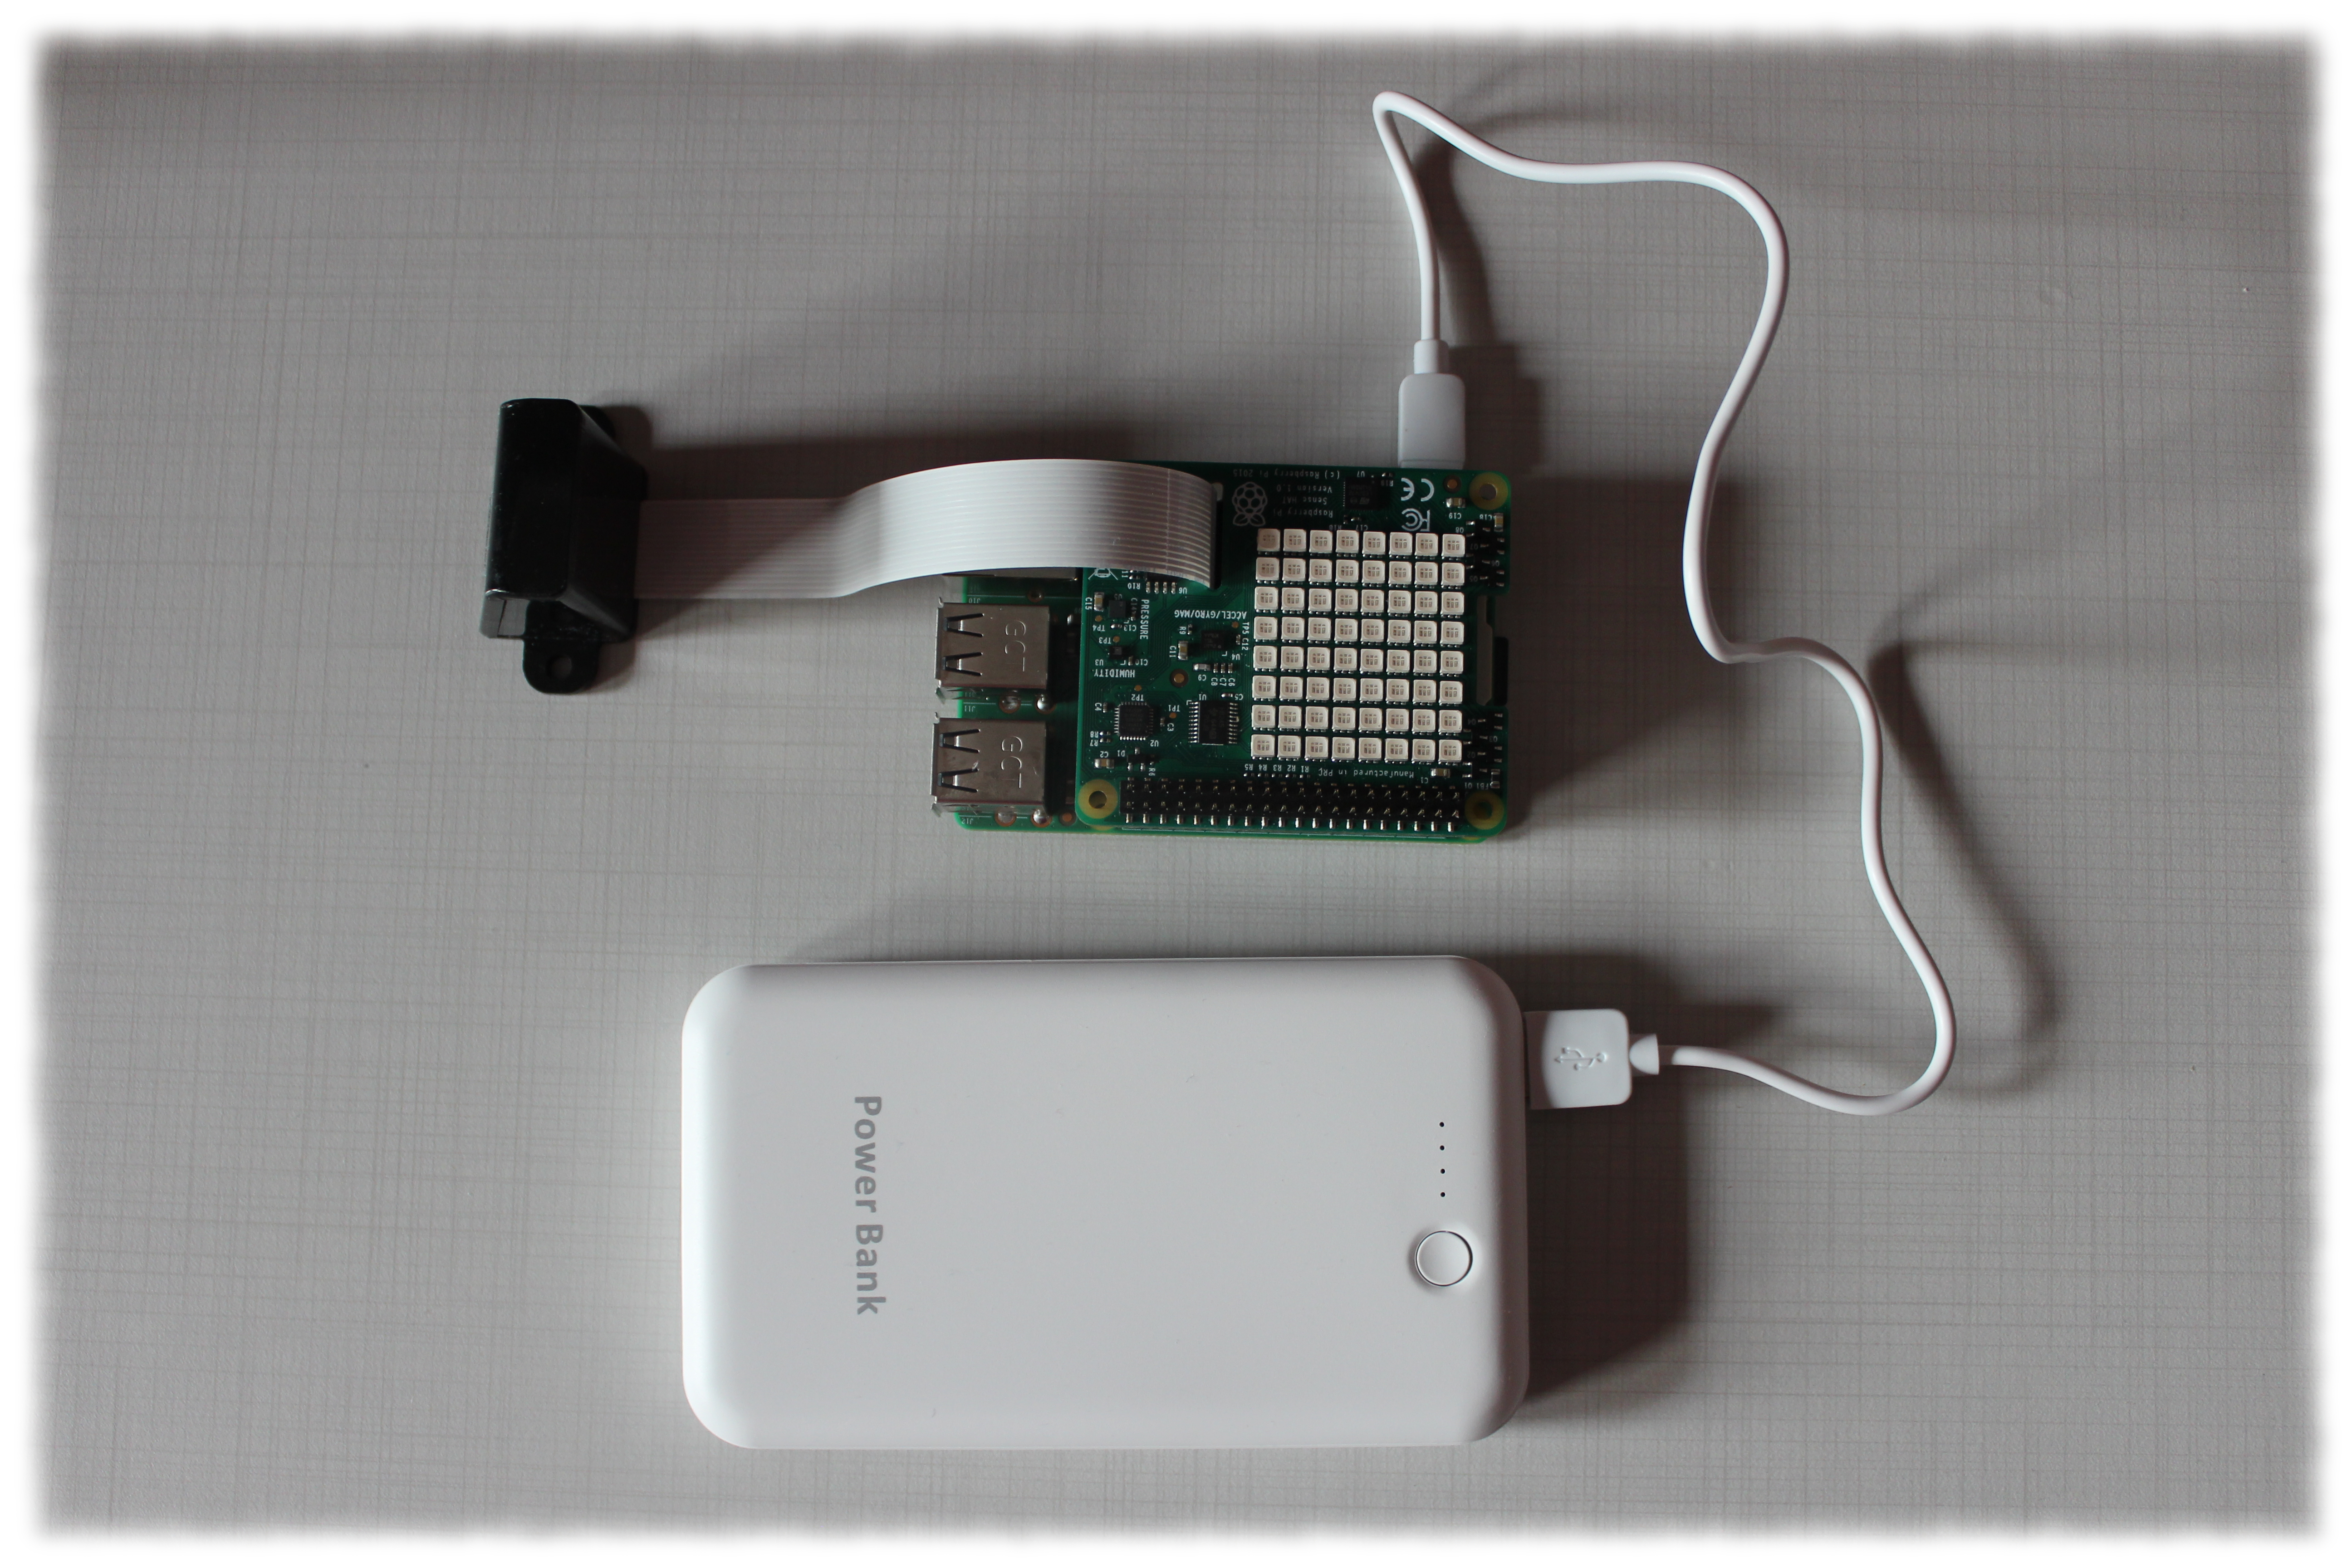
\includegraphics[width=0.8\textwidth]{6-Sistema_v1.jpg}
		\caption{Device structure with PiCamera installed}
		\label{fig:6-Sistema_v1}
	\end{center}
\end{figure}

A configuration file has been implemented which contains some variables that are used by several modules of the device. Hence, these values are stored only once and can be changed easily. The whole file is shown and explained in Appendix \ref{chap:user_manual}. The parameters related with the camera are shown in Listing \ref{lst:6-camera-config}.

\lstinputlisting[language=Python, firstline=1, texcl, caption = {Part of \texttt{config.py} file containing the camera parameters}, label = lst:6-camera-config]{code/6-camera-config.py}

To assure the correct functionality of the camera, some videos are recorded. For that purpose and following the examples provided in PiCamera documentation \cite{PiCameraDoc}, a script has been developed. This script is shown in Listing \ref{lst:6-camera-video-recording}. This script must wait two seconds to ensure the camera is initialized correctly, then the camera starts recording during 60 seconds (as it is defined in \texttt{config.py}) and finally the video is saved in the file \texttt{my\_video.h264} in h264 video format.

\lstinputlisting[language=Python, firstline=1, texcl, caption = {Sample recording with PiCamera script}, label = lst:6-camera-video-recording]{code/6-camera-video-recording.py}


\subsubsection{Extract the motion vectors when recording a video with the PiCamera module using PiMotionAnalysis and PiMotionArray}
The result of the previous task allows recording videos using the PiCamera. This task deals with the need of extracting the motion data from the videos. To achieve this task, \texttt{PiMotionAnalysis} class from \texttt{picamera.array} is used. While recording is in progress, the incoming motion data is converted into a numpy array and an analysis method is called with the resulting array passed as argument. This class can be extended and the analysis method can be overridden. Therefore, in this method, the motion vectors can be used to detect movement in the video.

\BLUENOTE{Due to the fact that this class is used when the video is being recorded, it is used in the final implementation but first, in order to realize the different test, another class is used instead. The reason is that in this early steps of the work, it is more interesting to have the videos with the motion data stored into files and use them at any time. Hence, \texttt{PiMotionArray} class is used, which converts the incoming motion data into a numpy array also, but the conversion its made when the recording has finished. The class generates a 3-dimensional numpy array organized as (frames, rows, columns) where rows and columns are the number of the rows and columns of the macro-block \REDNOTE{(reference to the explanation of a macro-block)} in the frame. There is an extra column in the motion vector data that is not going to be used. Then, the data is stored into a file. 
}

\begin{figure}[!h]
	\begin{center}
		\includegraphics[width=0.8\textwidth]{6-Car_with_MV.png}
		\caption{Example of  the motion vectors taken by the Raspberry Pi}
		\label{fig:6-Car_with_MV}
	\end{center}
\end{figure}

The class used for recording the videos and the motion vectors used for developing the algorithm to count cars can be shown in Listing \ref{lst:6-Recorder-Sprint1}. Some parameters are given as arguments: \texttt{distance} and \texttt{angle}. They are used only for the filename so as to know afterwards the conditions of the camera when the video was recorded. In this class, the camera is configured according to the values stored in \texttt{config.py}. When the video has been recorded, it will be stored in a file with extension \texttt{.h264}, as well as the motion data, that will be stored in a file with the same name and extension \texttt{.data}. To finish with, the video will be also converted to \texttt{.mp4} to make easier its view in the development computer. 

\REDNOTE{IMPORTANT NOTE: Image resizer is not used. An other option is configure the camera resolution to 1920x1080 and use a resizer in the video to reduce the resolution given to the H.264 video coder.}

\lstinputlisting[language=Python, firstline=1, texcl, caption = {Class used to record a video and its corresponding motion data}, label = lst:6-Recorder-Sprint1]{code/6-Recorder-Sprint1.py}

\subsubsection{Develop a noise filter using moving averages}
There are some factors that can affect the number of motion vectors in a certain frame. Some of these factors can be the incorrect codification of that frame or a small object crossing the image (e.g., a person or a bug). Moreover, when H.264 video coding is used, there are several types of frame: I-frames, P-frames and B-frames \REDNOTE{(reference to their explanation)}. I-frames do not require other video frames to be decoded, therefore, they do not generate any motion vectors. Thus, the number of motion vectors in some frames is not going to be close to the reality, causing noise. To solve this problem, a smoothing technique is used. More concretely, simple moving averages calculation is applied.

A simple moving average \cite{Smi15} is a unweighted average of k prior values. Since a time series can be regarded as a sequence of values, $\{\overline {x_{t}}\}$, being $t=1,2,3,4,…n$, the moving average of these values can be computed. If we assume that $n$ is quite large, and we select an integer $k$ which is much smaller than $n$, we can compute the simple moving averages (of order k) as shown in Equation (\ref{eq:simple_moving_averages}).

\begin{equation} \label{eq:simple_moving_averages}
\overline { { x }_{ t } } =\frac { 1 }{ k } \sum _{ i=t-k+1 }^{ t }{ { x }_{ i } } ,\quad 2\le k\le n
\end{equation}

The result of applying the simple moving average over the data recorded previously can be shown in Figure \ref{fig:6-moving_averages}. Here, it can be appreciate how the graphic corresponding with the data before applying simple moving averages (black line) has some noise and sometimes it falls to 0. Additionally, it can be shown how the problem is decreased using this smoothing technique.

\begin{figure}[!h]
	\begin{center}
		\includegraphics[width=1\textwidth]{6-moving_averages.pdf}
		\caption{Result of applying moving averages of order $n = 6$ to smooth the data}
		\label{fig:6-moving_averages}
	\end{center}
\end{figure}


\subsubsection{Develop the basic algorithm to counts the cars}
To count the cars that go across a street depending on its direction and using the motion data previously stored, an algorithm has been developed. Its pseudocode is shown in Algorithm \ref{alg:count_cars_V1}. This algorithm discriminates the cars direction (left or right). For each of the directions, the following algorithm is executed: 

For each frame, the number of motion vectors in that frame is compared with the number of vectors in the previous frame, increasing or decreasing a variable called \texttt{growth}. Once the number of frames exceed the \texttt{HEIGHT\_THRESHOLD} variable, if the \texttt{growth} variable is positive, the variable \texttt{n\_positive\_frames} is increased by one. If this last variable overtakes the \texttt{WIDTH\_THRESHOLD} variable, then it can be considererd that a new car has been detected. If the \texttt{growth} variable gets equal to \texttt{-GROWTH\_LIMIT}, then it is considered that the car has already passed, and the variable \texttt{n\_positive\_frames} is restored to its initial value (zero).

An example of the execution fo the algorithm can be shown in Figure \ref{fig:6-Count_cars_graphic}, where the blue line represents the number of motion vectors with left direction for each frame, and the red line represents the same but for right direction. The black line, represent the \texttt{HEIGHT\_THRESHOLD} variable. Therefore, a car can be predicted if the number of frames in one direction overtakes the \texttt{HEIGHT\_THRESHOLD} variable during more than \texttt{WIDTH\_THRESHOLD} frames. And, it can be considered that the car has already cross if the number of frames has been decreasing $\texttt{GROWTH\_LIMIT} \times 2 $ frames, regardless if the number of motion vectors is under the \texttt{HEIGHT\_THRESHOLD} variable or not. Therefore, in Figure \ref{fig:6-Count_cars_graphic}, it can be considered that two different cars have cross near the frame 1000, as the number of motion vectors has decreased during more than $\texttt{GROWTH\_LIMIT} \times 2 $ frames.

%\IncMargin{1em}
\begin{algorithm}
	\SetKwInOut{Input}{Input}\SetKwInOut{Output}{Output}
	\LinesNumbered
	\SetAlgoLined
	
	\Input{cols --> Number of colums with a macroblock in each frame\\
		rows --> Number of rows with a macroblock in each frame\\
		frames --> The number of frames in the video. \\
		motion\_data --> Array that contains a structure [x,y,SAD] for each frame} 
	\Output{n\_cars  --> Vector which contains the number of cars that has been counted crossing in left and right direction respectively.}
	
	n\_cars $\gets$ [0, 0]\;
	mv $\gets$ []\;
	smooth\_mv $\gets$ []\;
	car\_detected $\gets$ [False, False]\;
	growth $\gets$ [0, 0]\;
	n\_positive\_frames $\gets$ [0, 0]\;
	
	
	\For{frame $\gets$ 0 to frames}{
		%Add to the end of $mv$ vector a list with two elements. The first element consist in the number of motion vectors in that frame whose 'x' value is greather than the variable $GROUP\_SENSITIVITY$. The second element is the number of them whose 'x' value is lower than $-GROUP\_SENSITIVITY$.
		\tcc{Obtain number of motion vectors in each direction.}
		mv.append([ (motion\_data[frame]['x'] > GROUP\_SENSITIVITY).sum() ,
		(motion\_data[frame]['x'] < -GROUP\_SENSITIVITY).sum() ])\;
		
		\BlankLine
		\tcc{Apply moving averages to smooth the number of motion vectors}
		tmp\_left $\gets$ 0, tmp\_right $\gets$ 0\;
		\For{i $\gets$ 0 to SMOOT\_ORDER}{
			j $\gets$ frame - i\;
			\lIf{j < 0}{j $\gets$ 0}
			tmp\_left $\gets$ tmp\_left + mv[j][0] \;
			tmp\_right $\gets$ tmp\_right + mv[j][1]\;
		}
		smooth\_mv.append([tmp\_left / SMOOT\_ORDER, tmp\_right / SMOOT\_ORDER])\;
		
		\BlankLine
		\BlankLine
		\For{direction $\gets$ 0 to 2}{
			\uIf{smooth\_mv[frame-1][direction] < smooth\_mv[frame][direction]\\
				\hskip2em \textbf{and} growth[direction] < GROWTH\_LIMIT}{
				growth[direction] $\gets$ growth[direction] + 1\;
			}
			\ElseIf{smooth\_mv[frame-1][direction] < smooth\_mv[frame][direction]\\
				\hskip2em \textbf{and} growth[direction] > -GROWTH\_LIMIT}{
				growth[direction] $\gets$ growth[direction] - 1\;
			}
			
			\uIf{smooth\_mv[frame][direction] >= HEIGHT\_THRESHOLD \\
				\hskip2em \textbf{and} growth[direction] > 0}{
				n\_positive\_frames[direction] $\gets$ n\_positive\_frames[direction] + 1\;
				\If{n\_positive\_frames[direction] >= WIDTH\_THRESHOLD \\
					\hskip2em \textbf{and} car\_detected[direction] = False}{
					car\_detected[direction] $\gets$ True\;
					n\_cars[direction] $\gets$ n\_cars[direction] + 1\;
				}
				
			}
			\ElseIf{growth[direction] = -GROWTH\_LIMIT}{
				car\_detected[direction] $\gets$ False\;
				n\_positive\_frames[direction] $\gets$ 0\;
			}	
		}	
	}
	\caption{Count cars (First Version)}\label{alg:count_cars_V1}
\end{algorithm}\DecMargin{1em}

\begin{figure}[!h]
	\begin{center}
		\includegraphics[width=1\textwidth]{6-Count_cars_graphic.pdf}
		\caption{Number of motion vectors in the test video 8}
		\label{fig:6-Count_cars_graphic}
	\end{center}
\end{figure}

Once the algorithm has been developed, it should be tested using the different videos recorded previously as it was stated in the list of test for the user story. The result of executing the algorithm over the different videos is shown in Table \ref{tab:Results_CountCars_V1}. After evaluating the results obtained, it is concluded that they are acceptable for the goal of this Sprint, therefore, a new Sprint can be started.

\begin{table}[hp]
	\centering
	{\small
		\begin{tabular}{ |P{.08\textwidth}P{.15\textwidth}P{.15\textwidth}P{.2\textwidth}P{.15\textwidth}|}
	\hline
	\rowcolor{tabheadbg}
	\multicolumn{5}{|c|}{\textscale{.8}{\textbf{Algorithm \ref{alg:count_cars_V1} results}}} \\
	\hline
	\hline
	\textscale{.8}{\textbf{Number}} & \textscale{.8}{\textbf{Quality}} & \textscale{.8}{\textbf{Camera angle}} & \textscale{.8}{\textbf{Distance to the road}} & \textscale{.8}{\textbf{Percentage of hits}} \\
	\hline
	1 	& 1080x720		 	&  center 		& 1m	& \textbf{100\%} \\ 
	\hline
	2 	& 1080x720		 	&  center 		& 1m	& \textbf{100\%} \\ 
	\hline
	3 	& 1080x720		 	&  center 		& 1m	& \textbf{90\%} \\ 
	\hline
	4 	& 1080x720		 	&  center 		& 2m	& \textbf{90.91\%} \\ 
	\hline
	5 	& 1080x720		 	&  center 		& 2m	& \textbf{100\%} \\ 
	\hline
	6 	& 1080x720		 	&  center 		& 2m	& \textbf{100\%} \\ 
	\hline
	7 	& 1080x720		 	&  center 		& 2m	& \textbf{94.74\%} \\ 
	\hline
	8 	& 1080x720		 	&  center 		& 3m	& \textbf{100\%} \\ 
	\hline
	9 	& 1080x720		 	&  center 		& 3m	& \textbf{90.91\%} \\ 
	\hline
	10 	& 1080x720		 	&  left 		& 1m	& \textbf{86.67\%} \\ 
	\hline
	11	& 1080x720		 	&  left 		& 1m	& \textbf{100\%} \\ 
	\hline
	12 	& 1080x720		 	&  left 		& 1m	& \textbf{100\%} \\ 
	\hline
	13 	& 1080x720		 	&  left 		& 2m	& \textbf{100\%} \\ 
	\hline
	14 	& 1080x720		 	&  left 		& 2m	& \textbf{55.56\%} \\ 
	\hline
	15 	& 1080x720		 	&  left 		& 2m	& \textbf{73.33\%} \\ 
	\hline
	16 	& 1080x720		 	&  left 		& 2m	& \textbf{88.89\%} \\ 
	\hline
	17 	& 1080x720		 	&  right 		& 1m	& \textbf{66.67\%} \\ 
	\hline
	18 	& 1080x720		 	&  right 		& 1m	& \textbf{78.57\%} \\ 
	\hline
	19 	& 1080x720		 	&  right 		& 1m	& \textbf{90\%} \\ 
	\hline
	20 	& 1080x720		 	&  right 		& 2m	& \textbf{83.33\%} \\ 
	\hline
	21 	& 1080x720		 	&  right 		& 2m	& \textbf{91.67\%} \\ 
	\hline
	22 	& 1080x720		 	&  right 		& 2m	& \textbf{88.89\%} \\ 
	\hline
	23 	& 1080x720		 	&  right 		& 2m	& \textbf{90\%} \\ 
	\hline
	\hline
	\multicolumn{3}{|c|}{\textscale{.8}{\textbf{Total number of tests: }} 23} & \multicolumn{2}{|c|}{\textscale{.8}{\textbf{Global percentage of hits: }} \textbf{89.57\%}} \\
	\hline
	
\end{tabular}
	}
	\caption{Results of the Algorithm \ref{alg:count_cars_V1} over the first test dataset}
	\label{tab:Results_CountCars_V1}
\end{table}


\REDNOTE{Task: Create a module that use the counting algorithm to obtain the vehicle flow in real time (using PiMotionAnalysis) in this Sprint or in another one.}



%%% Sprint 2
\section{Sprint 2: Design of an environmental parameters monitoring system}
In this Sprint, a program to obtain environmental data is going to be developed. This involves the implementation of some environmental sensors to measure some parameters such as temperature, humidity and pressure, as well as, the design and implementation of an electronic circuit to measure some contaminant gases. These gas sensors are going to be MQ-7 and MQ-2 sensors, which measures CO and LPG gases respectively. Once the circuit has been implemented, some code must be developed in order to control the sensors, as well as get the data they generate and store it into a data structure.

\subsection{Sprint planning meeting}
During the planning meeting, the two user stories addressed in this sprint has been analysed. These user stories are shown in Tables \ref{tab:Sprint2-User-story-4} and \ref{tab:Sprint2-User-story-5}.

\UserStoryTable{4}{2}{High}{25}
{Install environmental and gas sensors into Raspberry Pi}
{Design and implement the electronic circuit to integrate the different sensors into Raspberry Pi device.}
{	\item Install Raspberry Pi Sense Hat board
	\item Design an electronic circuit for the MQ gas sensors
	\item Connect the electronic circuit to Raspberry Pi device
}{	\item Check if the sensors are working correctly
	\item Test the connectivity of the Raspberry Pi with the external electronic circuit
}

\UserStoryTable{5}{2}{High}{30}
{Obtain and process data from the sensors}
{Develop a module that allows to communicate with the installed sensors and obtain the data.}
{	\item Develop a class that communicates with the external sensors using \ac{SPI}
	\item Develop a method to convert from the read values of the MQ sensors to particles per million
	\item Calibrate the MQ sensors
	\item Develop a method to control the different sensors and collect all the data
}{	\item Test the environmental sensors
	\item Test the MQ gas sensor
}

%Table \ref{tab:Sprint2-User-story-4}

\subsection{Results of the development of the tasks}

\subsubsection{Install Raspberry Pi Sense Hat board}
The installation of this board is very simple, as the only step is to place it correctly on top of the Raspberry Pi, making sure that the GPIO pins (Figure \ref{fig:6-Raspberry-Pinout-En}) are correctly aligned before pressing down firmly so the board properly attaches to the Raspberry Pi.

\subsubsection{Design an electronic circuit for the MQ gas sensors}
Due to the necessity of measuring some gases such as CO or Liquefied Petroleum Gas (LPG), some external sensors are needed, which are MQ-7 and MQ-2 sensors respectively. The MQ sensors are inexpensive gas sensors that are sensitive for a range of gasses and are recommended especially for indoor use. As we only want to obtain an approximate value of the polluting gases concentration (because accurate sensors are very expensive and require complex calibration methods), it has been decided to use these inexpensive sensors. Moreover, these sensors are quite common, so they can be obtained in lot of specialized stores. They provide an analogue signal output, hence a conversion to a digital value must be carried out. For this purpose an \ac{ADC} is needed, therefore the MCP3008 chip has been used \cite{MCP3008}.

As a result of the complexity of incorporating the MQ sensor directly to the electronic circuit, a chip module, which is shown in Figure \ref{fig:6-MQ_Sensor}, has been used instead. This chip implements the connections to the MQ sensor and provide 4 external connections (voltage, ground, digital output and analogue output). The digital output is not going to be used, as it only provides a logical value (1 or 0) according to a gas concentration threshold. Therefore, the analogue output is used and the value is converted to a digital one using the \ac{ADC} chip.

\begin{figure}[!h]
	\begin{center}
		\includegraphics[width=0.5\textwidth]{6-MQ_Sensor.jpg}
		\caption{MQ sensor chip used}
		\label{fig:6-MQ_Sensor}
	\end{center}
\end{figure}

The implementation of the MQ-2 sensor is quite straightforward, however, the MQ-7 sensor require more attention. This is because MQ-7 sensor works in cycles of two phases: First the sensor is powered by 1.4 volts during 60 seconds. At the end of this phase, the results are read from the sensor and then a phase of 90 seconds starts where the sensor is heated with 5 volts (which allows the sensor to clean up for the next measurement). In the case of the MQ-2 sensor, the 5 volts which are necessary in order to power it can be supplied by the 5 volts power supply (Pin 4) of the GPIO interface as shown in Figure \ref{fig:6-Raspberry-Pinout-En}, which can supply up to 700 mA. In the case of the MQ-7 sensor, \ac{PWM} is going to be used to generate the 1.4 volts, but the GPIO pins used for the \ac{PWM} can only supply 50 mA. This sensor consume approximately 150 mA and therefore the Raspberry pin can burn. To solve this problem the LM317 chip has been used, which is a regulator capable of supplying more than 1.5 Amperes over an output-voltage range of 1.25 volts to 37 volts \cite{LM317}. By using LM317 chip, the current is drawn form the 5 volts power supply and the pin BCM 16 can be used without any problem for generating a \ac{PWM}.

\ac{PWM} is a modulation technique that allow generating waveforms of high frequencies and high precision \cite{DdlT16}, and it can be used to control the power supplied to electrical devices, such as motors. To generate a \ac{PWM} signal it is needed to define the period and the duty cycle (Figure \ref{fig:6-PWM-signal}). The period indicates duration of each cycle, whereas the duty cycle describes the proportion of the period in which the signal is in high power state (in this case 3.3 volts, which is voltage generated by the GPIO pins). The frequency (which is the inverse of the period) has been defined to $100 Hz$ which is enough, and taking this value into account the duty cycle has been defined to $14\%$ in order to obtain 1.4 volts and to $100\%$ to obtain the maximum voltage allowed by the LM317 chip (for the heating phase). The final circuit is shown in Figure \ref{fig:6-Circuit-Schematic}.

\begin{figure}[!h]
	\begin{center}
		\includegraphics[width=0.75\textwidth]{6-PWM-signal.png}
		\caption{PWM signal}
		\label{fig:6-PWM-signal}
	\end{center}
\end{figure}

The consequence of using the LM317 chip is that it has an internal drift that we have measured as approximately 1.8 volts and, consequently, only 3.2 volts can be generated using a 5 volts power supply. Since the 5 volts phase is only used to heat the sensor, there is not a big difference in the precision of the measurements, hence this solution is going to be accepted for this prototype. In a final implementation, two solutions can be implemented to solve this problem. The first one is to use a higher voltage power supply (which is a simple solution if the device is connected to the street lighting power supply). A second approach consist in implement a circuit using transistors to switch between 1.4 and 5 volts. This second solution has not been implemented as it exceeds the objectives of this \ac{BSc.} thesis.


% https://easyeda.com/editor
\begin{figure}[!h]
	\begin{center}
		\includegraphics[width=1\textwidth]{6-Circuit-Schematic.pdf}
		\caption{Circuit schematic}
		\label{fig:6-Circuit-Schematic}
	\end{center}
\end{figure}

\begin{figure}[htb]
	\centering
	\subfigure[Raspberry Pi Pinout Board Schema]{
		\includegraphics[height=0.82\textwidth,angle=90]{6-Raspberry-Pinout-En.png}
		\label{fig:6-Raspberry-Pinout-En}
	}
	\subfigure[Raspberry Pi Pinout Connections]{
		\includegraphics[width=1\textwidth]{6-Raspberry-Pinout-Expanded.png}
		\label{fig:6-Raspberry-Pinout-Expanded}
	}
	\caption{Raspberry Pi Pinout}
	\label{fig:6-Raspberry-Pinout}{Source: \url{https://pinout.xyz/}}
\end{figure}




\subsubsection{Connect the electronic circuit to Raspberry Pi device}
The next step is to connect the previous electronic circuit to the Raspberry Pi. For this purpose the GPIO pins are going to be used. However, as the Sense hat module has been installed in the Raspberry Pi, not all the GPIO pins are available. These pins can be located in Figure \ref{fig:6-Raspberry-Pinout-Expanded} or using the webpage \url{https://pinout.xyz/} where all the information about the different pins is displayed. Therefore, for the \ac{SPI} communication with the MCP3008 chip the pins BCM  18, 19, 20, and 21 are used. In addition, pin BCM 16 is used for \ac{PWM} and GPIO 4 and 6 for 5 volts power and ground respectively. Figure \ref{fig:6-Electric_diagram.pdf} shows the connection diagram of the components using a protoboard to connect them.

\begin{figure}[!h]
	\begin{center}
		\includegraphics[height=1\textwidth,angle=90]{6-Electric_diagram-cropped.pdf}
		\caption{Connection diagram of the components}{Image generated using fritzing}
		\label{fig:6-Electric_diagram.pdf}
	\end{center}
\end{figure}


\subsubsection{Develop a class that communicates with the external sensors using \ac{SPI}}
As it has been previously commented, the analogue output from the MQ sensors will be converted to a digital value using an \ac{ADC} chip. For this purpose, the MCP3008 chip \cite{ADC} is going to be used, which communicates with the processor using \ac{SPI} protocol. The class developed need to implement this protocol internally in order to obtain the data form this chip using the GPIO pins (Listing \ref{lst:6-spiCommunicator}). The protocol has been implemented following the specifications of the MCP3008 datasheet, where all the signals that need to be activated in each clock cycle are stated. The channel is going to be provided as argument, being channel 0 the MQ-7 sensor and channel 1 the MQ-2 sensor, as it was stated in the wiring connections of Figure \ref{fig:6-Circuit-Schematic}.

\begin{figure}[!h]
	\begin{center}
		\includegraphics[width=0.9\textwidth]{6-MCP3008-SPI.pdf}
		\caption{Communication with SCP3008}{Image from MCP3008 datasheet \cite{ADC}}
		\label{fig:6-MCP3008-SPI}
	\end{center}
\end{figure}

\lstinputlisting[language=Python, firstline=27, texcl, caption = {\emph{read} method from \texttt{spiCommunicator.py} file}, label = lst:6-spiCommunicator]{code/6-spiCommunicator.py}


\subsubsection{Develop a method to convert from the read values of the MQ sensors to particles per million}
The values provided by the previous class corresponds to the voltage of the current that goes through the sensor and it need to be converted to particles per million of the gas measured. For this purpose the sensitivity characteristic curve of the different gases (Figure \ref{fig:6-MQ_curve}) defined in the sensor documentation must be studied. This curve explains how the resistance of the sensor changes depending on the concentration of the target gas. Therefore, the first step must be calculating the resistance of the sensors. 

The value provided by the \ac{SPI} protocol need to be converted in order to obtain the real value of the voltage. In the MCP3008 chip documentation \cite{ADC} the Equation \ref{eq:digital_output_code_calculaiton} is purposed to calculate the value given by the converter ($adc$), where ${V}_{RL}$ is the value of the voltage being measured in the corresponding channel of the converter and ${V}_{R}$ the reference level used by the converter.
\begin{equation} \label{eq:digital_output_code_calculaiton}
adc = \frac { 1024\cdot { V }_{ RL } }{ { V }_{ R } } 
\end{equation}
This equation can be modified to obtain the real value of the voltage going through the gas sensor, as shown in Equation \ref{eq:VRL}.
\begin{equation} \label{eq:VRL}
{ V }_{ RL } =\frac { adc \cdot  { V }_{ R }}{ 1024 }  
\end{equation}

The reference level used by the \ac{ADC} chip is going to be the same as the used for the rest of the circuit (5 Volts), as shown in Equation \ref{eq:ref_voltage}.
\begin{equation} \label{eq:ref_voltage}
{V}_{R} = {V}_{C}
\end{equation}

To obtain the resistance of the MQ sensors, their official documentation \cite{MQ7,MQ2} purpose the use of the Equation \ref{eq:operational_principle}, where ${R}_{S}$ is the current resistance of the sensor (in $K\Omega$, i.e. 1000 ohms), ${R}_{L}$ is the load resistance in $K\Omega$ (i.e. the external resistance connected to the sensor) and ${V}_{RL}$ is the value of the voltage being measured. 
\begin{equation} \label{eq:operational_principle}
{ { R }_{ S } }/{ { R }_{ L } }=\frac { { V }_{ C }-V_{ RL } }{ V_{ RL } } 
\end{equation}

Combining Equations \ref{eq:VRL}, \ref{eq:ref_voltage} and \ref{eq:operational_principle}, the final Equation \ref{eq:Rs_equation} is obtained, which allows us to calculate the value of the MQ gas sensor resistance using the raw value obtained by the \ac{ADC} chip (denoted as $adc$).
\begin{equation} \label{eq:Rs_equation}
\begin{aligned}
{ { R }_{ S } }/{ { R }_{ L } }=\frac { { V }_{ C }-V_{ RL } }{ V_{ RL } } \Rightarrow 
{ { R }_{ S } }/{ { R }_{ L } }=\frac { { V }_{ C }-\frac { adc\cdot { V }_{ C } }{ 1024 }  }{ \frac { adc\cdot { V }_{ C } }{ 1024 }  } \Rightarrow \\
{ { R }_{ S } }/{ { R }_{ L } }=\frac { 1024\cdot { V }_{ C }-adc\cdot { V }_{ C } }{ adc\cdot { V }_{ C } } \Rightarrow 
{ R }_{ S }=\frac {  { R }_{ L } \cdot (1024-adc) }{ adc } 
\end{aligned}
\end{equation}

Listing \ref{lst:6-getResistance} shows the implementation of the previous equation into python code.
\lstinputlisting[language=Python, firstline=1, texcl, caption = {\emph{getResistance} method from \texttt{Sensors.py} file}, label = lst:6-getResistance]{code/6-getResistance.py}

To avoid outliers caused by some incorrect measurements, the final value of the resistance will be taken as the mean value of \texttt{READ\_SAMPLE\_TIMES} samples taken each \texttt{READ\_SAMPLE\_INTERVAL} milliseconds at shown in Listing \ref{lst:6-Read}.

Once the value of the MQ sensor resistance is known, the second step will be to convert it to particles per million (ppm). In order to achieve it, the corresponding MQ characteristic curve defined in its documentation must be implemented. For the purposes of simplicity, instead of defining the logarithm curved defined in the documentation, base ten logarithms will be taken in order to obtain a straight line and simplify the calculations, as it is shown in Figure \ref{fig:6-MQ_curve}. The abscissa axis represent the ppm concentration of the target gas, whereas the ordinate axis represent the ${R}_{S}/{R}_{O}$ quotient, where ${R}_{S}$ is the resistance of the sensor calculated in Equation \ref{eq:Rs_equation} and ${R}_{O}$ is the resistance of the sensor (calculated with the same equation) at a certain concentration of the gas that depends on the sensor. This ${R}_{O}$ parameter need to be adjusted for every sensor, as it is used to calibrate the measurements.

\begin{figure}[htb]
	\centering
	\subfigure[MQ-7]{
		\includegraphics[width=0.48\textwidth]{6-MQ-7_curve.png}
		\label{fig:6-MQ-7_curve}
	}
	\subfigure[MQ-2]{
		\includegraphics[width=0.48\textwidth]{6-MQ-2_curve.png}
		\label{fig:6-MQ-2_curve}
	}
	\caption{Sensitivity characteristic curve of the MQ sensors}
	\label{fig:6-MQ_curve}{Source: MQ sensor documentation \cite{MQ7,MQ2}}
\end{figure}

Therefore, to convert from the sensor resistance to ppm, the slope and the y-intercept of the line must be calculated for both sensors \cite{ConfMQX}. For example, to calculate the line that defines the CO concentration in the MQ-7 sensor, first, it is needed to calculate the slope of the line as shown in Equation \ref{eq:CO_slope}.
\begin{equation} \label{eq:CO_slope}
m=\frac { { y }_{ 2 }-{ y }_{ 1 } }{ { x }_{ 2 }-{ x }_{ 1 } } =\frac { \log _{ 10 }{ 0.09 } -\log _{ 10 }{ 1.8 }  }{ \log _{ 10 }{ 4000 } -\log _{ 10 }{ 50 }  } =-0.68
\end{equation}
The next step is to calculate the y-intercept of the line. Then, the left point of the line is taken and the base ten logarithm is applied, giving as a result the point $(x=1.7, y=0.26)$. These calculations must be repeated for the LPG measured by the MQ-2 sensor.

Now the line is calculated, the methods to convert from resistance to ppm can be developed as shown in Listing \ref{lst:6-getMQPPM}.

\lstinputlisting[language=Python, firstline=1, texcl, caption = {\emph{getMQPPM} method from \texttt{Sensors.py} file}, label = lst:6-getMQPPM]{code/6-getMQPPM.py}

The last step is to develop a method to obtain the final value from the sensor given the channel where it is connected. This method is shown in Listing \ref{lst:6-Read}

\lstinputlisting[language=Python, firstline=1, texcl, caption = {\emph{read} method from \texttt{Sensors.py} file}, label = lst:6-Read]{code/6-Read.py}


\subsubsection{Calibrate the MQ sensors}
The MQ sensor documentation purpose as a calibration method to generate a certain concentration of a given gas and measure the resultant resistance of the sensor. For example, for MQ-7 sensor, a concentration of 100ppm of CO in clean air is needed. Nevertheless, we have not enough resources to generate this gas concentration, and other calibration methods have been studied, such as measuring the current concentration of the gas with another CO sensor and compare the results, but it was not possible either. 

Therefore, an alternative approach have been developed in order to obtain an approximate value for ${R}_{O}$. It consists in locating the sensor into clean air (with not or not much CO and LGP contamination) and then measure the sensor resistance (${R}_{S}$). Then, the sensitivity curve of clean air for the given sensor can be calculated and used to obtain ${R}_{O}$, as shown in lines 16-19 of Listing \ref{lst:6-MQCalibration}, where \texttt{MQ\textbf{X}\_RO\_CLEAN\_AIR\_FACTOR} is the value of the clean air on the ordinate axis for the sensor sensitivity characteristic curve (Figure \ref{fig:6-MQ_curve}). This calculation will be repeated a certain number of times in order to obtain more accurate values. These steps have to be repeated for all units installed of each sensor type (MQ-7 and MQ-2), as the values changes depending on every sensor.

\lstinputlisting[language=Python, firstline=1, texcl, caption = {\emph{calibration} method from \texttt{Sensors.py} file}, label = lst:6-MQCalibration]{code/6-MQCalibration.py}

With this approach an approximate value of the gas concentration can be obtained, which is enough for this \ac{BSc.} thesis. Nonetheless, in a real implementation the sensor must be correctly calibrated, in order to obtain the real gas concentration.


\subsubsection{Develop a method to control the different sensors and collect all the data}

In order to control and collect the data from all the previous sensors a new method have to be developed. Firstly, the necessary GPIO pins for the sensors are going to be configured, as well as the \ac{PWM} cycle for controlling the voltage of the MQ-7 sensor is going to be initialized. Secondly, all the sensor data form the MQ sensors and from the environment sensors installed in the Sense Hat \cite{SenseHAT} are going to be obtained.

In order to avoid noisy data or sudden changes on the data, a smoothed average is going to be applied as it is shown in Equation \ref{eq:smoothed_average}, where ${w}_{t+1}$ represents the actual data read by the sensor, $\overline{{w}_{t}}$ is the value calculated by the equation in the previous measure and $\alpha$ is a factor that indicates how much new values affect to the final value represented as $\overline{{w}_{t+1}}$.
\begin{equation} \label{eq:smoothed_average}
\overline { { w }_{ t+1 } } =\alpha \cdot { w }_{ t+1 }+(1-\alpha )\cdot \overline { { w }_{ t } } 
\end{equation}
The $\alpha$ coefficient must be calculated in order to make the influence of the $n^\text{th}$ previous measurement negligible. Therefore, Equation \ref{eq:epsilon} can be demonstrated from the previous one, where the maximum influence of the $n^\text{th}$ previous measurement ($\varepsilon$) is calculated.
\begin{equation} \label{eq:epsilon}
{ (1-\alpha ) }^{ n }<\varepsilon  
\end{equation}
If we suppose that $\varepsilon$ is negligible with a value of ${10}^{-3}$, and we only want that the last half hour has influence over the data taking the values from the sensors each 2.5 minutes, then $n$ must be 12. We can operate on the previous equation to obtain the Equation \ref{eq:gamma_value}.
\begin{equation} \label{eq:gamma_value}
{ (1-\alpha ) }^{ n }<\varepsilon \Rightarrow 1-\alpha <\sqrt [ n ]{ \varepsilon } \Rightarrow 1-\sqrt [ n ]{ \varepsilon }<\alpha
\end{equation}
Then, considering $n=12$ and $\varepsilon={10}^{-3}$, the value calculated is $\alpha=0.57$, which is the one that will be used.

These parameters are going to be used to adjust Equation \ref{eq:smoothed_average} obtaining the final equation. At this point, the Sprint has been completely finished and the Raspberry Pi device can obtain not only environmental and pollution information, but also the traffic flow as it was explained in section \ref{Section:Sprint1}.


%%% Sprint 3
\section{Sprint 3: Development a module to send data from Raspberry Pi to the cloud and store it into a Database}
\REDNOTE{...}
% Product Backlog refinement

\subsection{Sprint planning meeting}
\REDNOTE{...}

%\UserStoryTable{6}{3}{High}{x}
%{Name of the user story}
%{A description of the user story}
%{	\item Task A
%	\item Task B
%	\item Task C
%}{	\item Test A
%	\item Test B
%}

%Table \ref{tab:Sprint2-User-story-4}

\subsection{Results of the development of the tasks}
\textbf{task something ...}

\REDNOTE{...}


%%% Sprint 4
\section{Sprint 4: Development of a program to monitor the data in real time and control the Raspberry Pi systems}
\REDNOTE{...}
% Product Backlog refinement

\subsection{Sprint planning meeting}
\REDNOTE{...}

%\UserStoryTable{4}{3}{High}{x}
%{Name of the user story}
%{A description of the user story}
%{	\item Task A
%	\item Task B
%	\item Task C
%}{	\item Test A
%	\item Test B
%}

%Table \ref{tab:Sprint2-User-story-4}

\subsection{Results of the development of the tasks}
\textbf{task something ...}

\REDNOTE{...}



%%%% Sprint X
%\section{Sprint X: ....}
%\REDNOTE{...}
%% Product Backlog refinement
%
%\subsection{Sprint planning meeting}
%\REDNOTE{...}
%
%%\UserStoryTable{4}{3}{High}{x}
%%{Name of the user story}
%%{A description of the user story}
%%{	\item Task A
%%	\item Task B
%%	\item Task C
%%}{	\item Test A
%%	\item Test B
%%}
%
%%Table \ref{tab:Sprint2-User-story-4}
%
%\subsection{Results of the development of the tasks}
%\textbf{task something ...}
%
%\REDNOTE{...}
%
%\subsection{Daily Scrum}
%\REDNOTE{...}
%
%\subsection{Sprint review}
%\REDNOTE{...}
%
%\subsection{Sprint retrospective}
%\REDNOTE{...}

% TFG - José Ángel Martín Baos. Escuela Superior de Informática. 2017
%%%% CHAPTER: Conclusiones %%%
\chapter{Conclusiones} %TODO
\label{chap:conclusiones}

% \drop{I}{n}


% Ideas:
% Reflexionar sobre los principales hitos conseguidos. Comparativa objetivos planteados vs objetivos consegudios
% Plantear trabajo futuro -> Posibles mejoras o amplificaciones del TFG
% Reflexión sobre los conocimientos adquiridos ?


\quoteauthor{\textcolor{red}{Ciudad Real, XX de Mayo de 2018}} %TODO
\quoteauthor{José Ángel Martín Baos}


%%%% CHAPTER: Conclusions %%%
\chapter{Conclusions} %TODO
\label{chap:conclusions} 






\quoteauthor{\textcolor{red}{Ciudad Real, XX May 2018}} %TODO
\quoteauthor{José Ángel Martín Baos}


\appendix
\appendixtitle
% TFG - José Ángel Martín Baos. Escuela Superior de Informática. 2018
%%%% CHAPTER: Installation Guide %%%
% !TeX spellcheck = en_GB

\chapter{Installation guide} % TODO: Revise all
\label{chap:installation_guide}

\drop{I}{n} this appendix, the steps to install and configure the Raspberry Pi device in order to execute the software developed in this project are explained. Raspbian \ac{OS} \cite{Raspbian} is the Operative System that will be installed on the Raspberry Pi. Raspbian is an modification of Debian \ac{OS} for Raspberry Pi and ARM processors. In this installation guide, a GNU/Linux Operating System has been employed in the personal computer.


\section{Installation and configuration of Raspbian}
The first step to get the device working consists in the installation of the Raspbian Operating System and the configuration of the device to allow us access the Raspberry from another device using a wireless connection.

\subsection{Installation of Raspbian in a SD card}
There are two main alternatives to install Raspbian in the Raspberry Pi. The first one consists in downloading the \ac{OS} image and extracting it into the SD card, which is the method explained here. The second form, which is recommended for people with lower knowledge on Linux \ac{OS}, consists in downloading the NOOBS software. This software has to be copied into the SD card and when the Raspberry Pi is executed for the first time an installation process will be carried out and Raspbian will be installed. 

Raspbian \ac{OS} can be downloaded from the Raspberry Pi downloads page\footnote{Raspbian download page: \url{https://www.raspberrypi.org/downloads/raspbian/}}. Once downloaded, the following steps should be followed in order to have Raspbian properly working on the Raspberry Pi board:
\begin{enumerate}
	\item Download Raspbian and check the download. To check if the download has been correctly carried out, the following command has to be executed, where \emph{file.zip} is the downloaded file and \emph{hash\_value} is the SHA-1 value for the downloaded file which can be found on the download page.
\begin{console}
$ sha1sum file.zip | grep hash_value
\end{console} %$

	\item Now, the mirco-SD card can be inserted and mounted on the computer. Usually the card gets mounted automatically. The list of devices mounted on the computer is shown in the Figure \ref{fig:Appendix_df-h_command}. Here, it can be observed that the mirco-SD card correspond to the route \texttt{/dev/sdb1}. The command used is: 
\begin{console}
$ df -h
\end{console} %$
	\begin{figure}[!h]
		\begin{center}
			\includegraphics[width=0.9\textwidth]{Appendix_df-h_command.png}
			\caption{\texttt{df -h} command execution}
			\label{fig:Appendix_df-h_command}
		\end{center}
	\end{figure}

	\item Once the path where mirco-SD has been mounted is known, the next step is to execute the following command to unmount the card, where \texttt{/dev/sdb1} is de route corresponding to your card. This avoids that the \ac{OS} writes the card while the files are being copied.
\begin{console}
$ umount /dev/sdb1
\end{console} %$

	\item Now, the \ac{OS} image can be extracted and copied to the micro-SD card as shown in Figure \ref{fig:Appendix_SO_copy}. The following commands have to be executed from the directory where the file has been downloaded:
\begin{console}
$ unzip 2017-07-05-raspbian-jessie.zip 
$ sudo dd bs=4M if=2017-07-05-raspbian-jessie.img of=/dev/sdb1
\end{console} %$

	\begin{figure}[!h]
		\begin{center}
			\includegraphics[width=0.9\textwidth]{Appendix_SO_copy.png}
			\caption{Console screenshot that shows the \ac{OS} copy process}
			\label{fig:Appendix_SO_copy}
		\end{center}
	\end{figure}

	\item Once the process has finished and before extracting the micro-SD card from the computer it should be ensured that the cache is clean. The next command must be executed:
\begin{console}
$ sync
\end{console} %$
	
\end{enumerate}


\subsection{Configuring Raspbian}
At this moment, the Raspbery Pi can be turned on. But firstly, it has to be connected to a external monitor or a TV using a HDMI cable. Nonetheless, this way is not very practical, therefore, some methods for allowing remote connection are explained. 

The first method consists in using \emph{ssh} protocol to access the Raspbery device. This protocol allows operating network services securely over an unsecured network. In others words, this method allows executing commands on the Raspberry Pi using a console, provided that the Raspberry Pi and the computer from where it is accessed are connected to the same network. OpenSSH tool \cite{OpenSsh} is installed with Raspbian \ac{OS} to provide the \emph{ssh} service. To activate it the following command should be executed:
\begin{console}
$ sudo raspi-config
\end{console} %$
This command executes the Raspbian configuration tool (Figure \ref{fig:Appendix_raspi-config_main}). \emph{Interfacing options} has to be selected. Using the new menu (Figure \ref{fig:Appendix_raspi-config_ssh}) SSH service should be selected and activated. Finally, the Raspberry Pi must be rebooted.

At this moment, the Raspberry Pi can be accessed from any computer connected to the same network using the next command, where \texttt{ipaddress} is the IP address of the network interface of the Raspberry Pi.
\begin{console}
$ ssh pi@ipaddress
\end{console} %$


The second method, consists in using a graphic remote session. VNC\footnote{VNC proyect main page: \url{http://www.hep.phy.cam.ac.uk/vnc_docs/index.html}} can be installed. VNC stands for Virtual Network Computing. It is, in essence, a remote display system which allows the user to view a computing 'desktop' environment, not only on the machine where it is running, but from anywhere on the Internet and from a wide variety of machine architectures. 

To activate VNC, the Interfacing options of the \texttt{raspi-config} tool has to be opened again as show in Figure \ref{fig:Appendix_raspi-config_ssh}. Then, VNC has to be selected and activated. Finally, the Raspberry Pi must be rebooted.

\begin{figure}[!h]
	\centering
	\subfigure[Main menu]{
		\includegraphics[width=0.48\textwidth]{Appendix_raspi-config.png}
		\label{fig:Appendix_raspi-config_main}
	}
	\subfigure[Interfacing Options]{
		\includegraphics[width=0.48\textwidth]{Appendix_raspi-config_ssh.png}
		\label{fig:Appendix_raspi-config_ssh}
	}
	\caption{Screenshot of raspi-config tool}
	\label{fig:Appendix_raspi-config}
\end{figure}

To access the \textsc{vnc} server executing in the Raspberry Pi, we have opted for using \textsc{vnc} viewer for Google Chrome, which is a version of \textsc{vnc} Connect\footnote{RealVNC main page: \url{https://www.realvnc.com/en/}} application adapted to execute in Google Chrome web browser. A screenshot of the program can be shown in Figure \ref{fig:Appendix_VNC-Viewer-Chrome}.

\begin{figure}[!h]
	\begin{center}
		\includegraphics[width=1\textwidth]{Appendix_VNC-Viewer-Chrome.png}
		\caption{Screenshot of \textsc{vnc} Viewer for Google Chrome.}
		\label{fig:Appendix_VNC-Viewer-Chrome}
	\end{center}
\end{figure}

The last step in this configuration process is to update the Raspbian \ac{OS} and applications. To accomplish this task, first, the filesystem should be expanded. This means that all the free space in the SD card will be available to the \ac{OS}. Again, the raspberry configuration tool has to be executed (Figure \ref{fig:Appendix_raspi-config_main}), and the \emph{Advance Options} menu has to be opened. Then, the \emph{Expand Filesystem} option must be selected. To finish with, the following commands have to be executed to update Rasbian:
\begin{console}
$ sudo apt-get update
$ sudo apt-get upgrade
\end{console} %$


\section{Installation of the necessary hardware and software}
Once we have the Raspberry Pi configured, it is needed to install some basic software and configure the hardware. In this case, as Python 3 had been used to develop the program that runs into the Raspberry Pi, Python 3 package installer (known as PIP) is needed. This software allows to install Python 3 packages easily. The next command has to be executed:
\begin{console}
$ sudo apt-get install python3-pip
\end{console} %$

\subsection{Installation of the PiCamera module}
In this project, the \emph{Raspberry Pi camera module V2} \footnote{More information about the Raspberry Pi camera module can be found in: \url{https://www.raspberrypi.org/products/camera-module-v2/}} is used. PiCamera \cite{PiCameraDoc} library is used to manage the Raspberry Pi camera installed. This library can be found on the Raspbian repositories, so it can be installed easily using the \emph{apt-get} command:
\begin{console}
$ sudo apt-get install python3-picamera
\end{console} %$

The next step is to enable the camera connection. The raspberry configuration tool will be executed (Figure \ref{fig:Appendix_raspi-config_main}), and the \emph{Interfacing options} menu should be opened. There, \emph{Camera} must be selected and activated. Then, the system should be restarted. Is important to know that the camera may not work well if there is not at least 128 MB of memory asignated to the \textsc{gpu}.

The last step is to connect the camera to the Raspbery Pi. The \textsc{csi} port must be used for this purpose. This port is located between the \textsc{hdmi} port and the stereo plug. It is advisable that when the camera is being installed the Raspberry must be turned off to avoid any damage to the camera. When connecting it, the blue part of the bus must be facing the stereo plug and the Ethernet connection as it is shown in Figure \ref{fig:Appendix_camera_conection}. 

\begin{figure}[!h]
	\begin{center}
		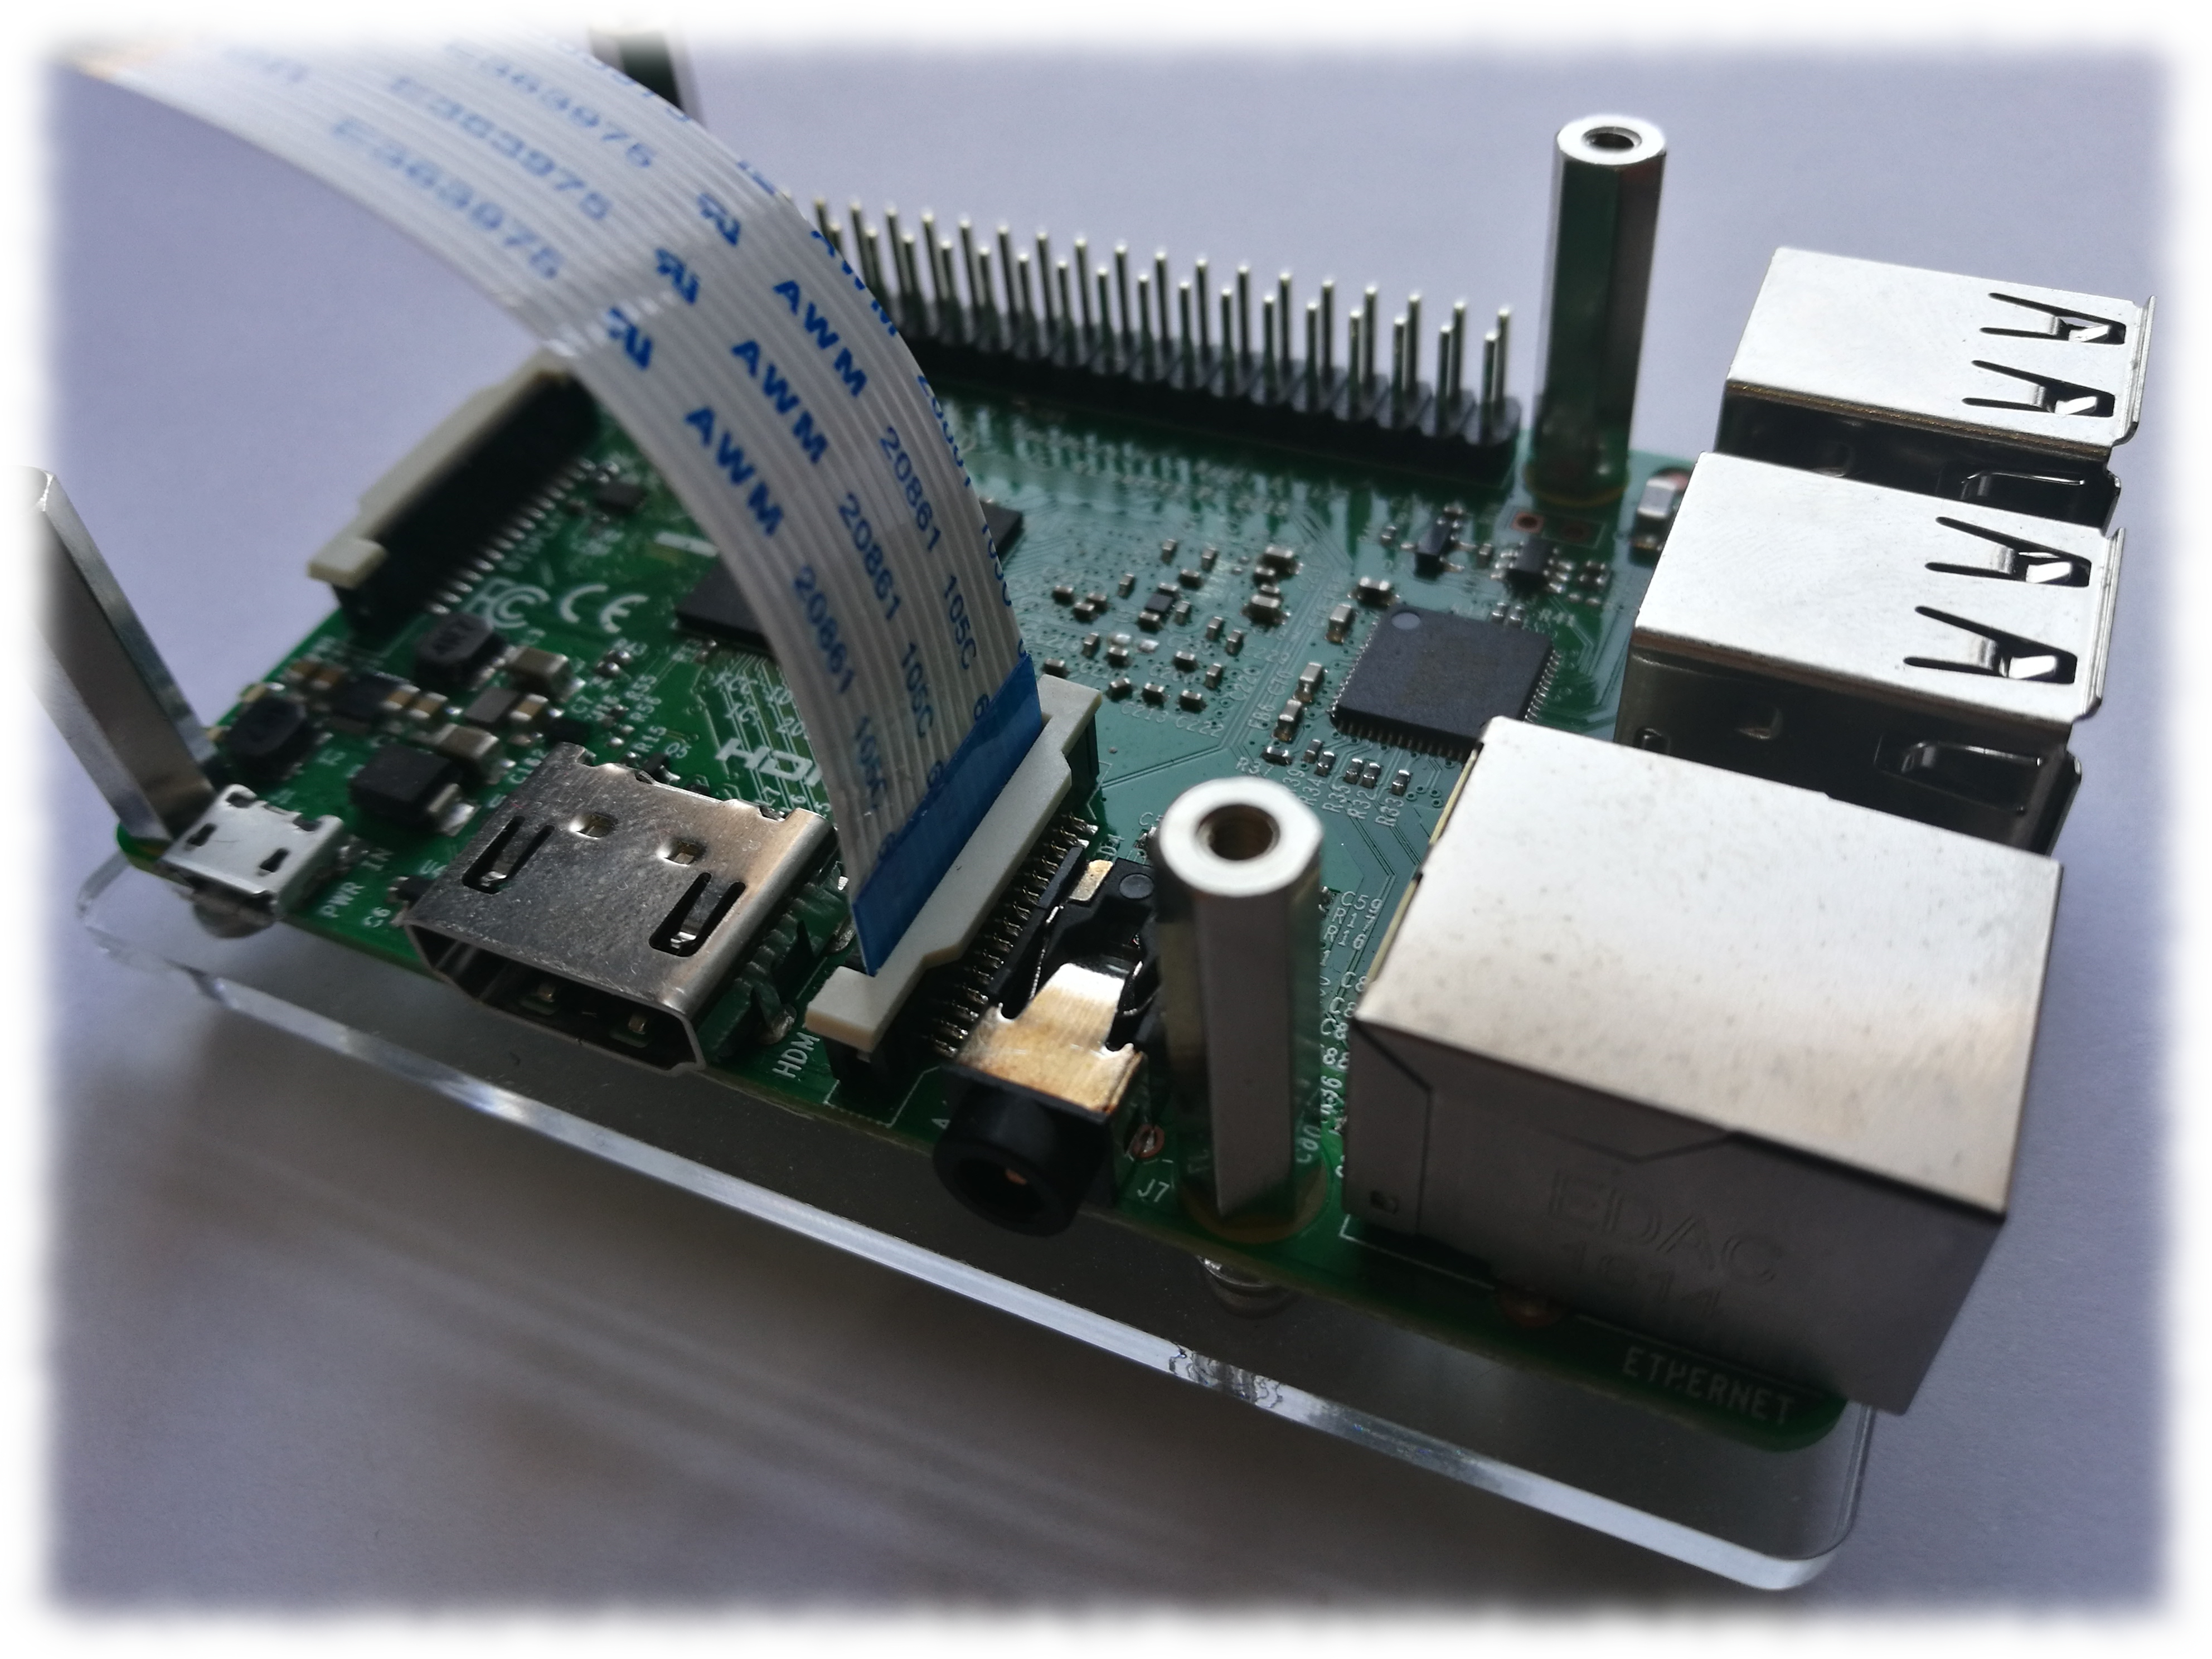
\includegraphics[width=0.75\textwidth]{Appendix_camera_conection.jpg}
		\caption{Connection of the camera module to the Raspberry Pi 3.}
		\label{fig:Appendix_camera_conection}
	\end{center}
\end{figure} %TODO: Cambiar imagen ?


\subsection{Installation of the sense hat}
The installation of the sense hat is explained on Task T2.4.1 of the Sprint 2 on the  \nameref{chap:results} chapter.

\subsection{Installation of the sensors}
The installation of the sense hat is explained on Tasks T2.4.2 and T2.5.1 of the Sprint 2 on the  \nameref{chap:results} chapter.


\subsection{Installation of the necessary libraries}
Some libraries are needed in order to execute the software developed in this \ac{BSc.} thesis:
\begin{enumerate}
	\item NumPy. Is the fundamental package for scientific computing with Python. NumPy can also be used as an efficient multi-dimensional container of generic data. To install it, the next command has to be executed:
\begin{console}
$ sudo apt-get install python-numpy python3-numpy
\end{console} %$

	\item Matplotlib. Is a library for the generation of graphic from data contained in list or arrays using Python programming language and the NymPy package. It provides a MATLAB-like interface. To install it, the next command has to be executed:
\begin{console}
$ sudo apt-get install python-matplotlib python3-matplotlib
\end{console} %$

	\item MP4Box. It can be used for performing many manipulations on multimedia files like AVI, MPG, TS, but mostly on ISO media files (e.g. MP4, 3GP). The justification for using it is that PiCamera generates the video recordings in \emph{h265} format. Therefore, this tool is used to convert videos from \emph{h265} to \emph{mp4}. The installation is done by executing the command:
\begin{console}
$ sudo apt-get install gpac
\end{console} %$
	Once installed, any video (named \texttt{video.h264}) can be converted from \emph{h265} to \emph{mp4} at 30 \ac{FPS} using:
\begin{console}
$ MP4Box -fps 30 -add video.h264 video.mp4
\end{console} %$

	\item Sense hat. To allow Raspberry Pi access the Sense Hat module, the corresponding library has to be installed:
\begin{console}
	$ sudo apt-get install sense-hat
\end{console} %$

	\item IBM Watson \ac{IoT} Platform. Some libraries are needed to allow Python to use the IBM Watson \ac{IoT} Platform services, which are used to send the sensor data to the Cloud. These libraries can be installed by executing the following commands:
\begin{console}
	$ sudo pip3 install ibmiotf
\end{console} %$

\end{enumerate}

When all these steps are completed, the Raspberry Pi is prepared for the correct execution of the software developed in this \ac{BSc.} thesis.

% TFG - José Ángel Martín Baos. Escuela Superior de Informática. 2018
%%%% CHAPTER: User Manual %%%
% !TeX spellcheck = en_GB
\chapter{Configuration file}
\label{chap:config_file}

\drop{I}{n} Appendix B the configuration file required by the program developed for the Raspberry Pi is explained. This configuration file is shown in Listing \ref{lst:B-config}, where lines from 1 to 18 define the Camera module configuration, lines from  21 to 70 define the Sensor module configuration, and lines from 73 to 75 define the communication module configuration.


\lstinputlisting[language=Python, texcl, firstline=11, texcl, caption = {Raspberry Pi program \texttt{config.py} file.}, label = lst:B-config]{code/B-config.py}


\backmatter
\bibliography{main}
\cleardoublepage

\end{document}
